\chapter[Интегративное моделирование с применением данных экспериментов по футпринтингу ДНК]{Интегративное моделирование с применением данных экспериментов по футпринтингу ДНК\footnote{При подготовке данного раздела диссертации использованы следующие публикации, выполненные автором лично или в соавторстве, в которых, согласно Положению о присуждении ученых степеней в МГУ, отражены основные результаты, положения и выводы исследования: \cite{shaytan_hydroxyl-radical_2017,shaytan_structural_2018,armeev_modeling_2016}.}} \label{part5_hrf}
%NAR
%Nature protocols
В данной главе обсуждаются подходы по моделированию ДНК-белковых комплексов, основанные на использовании экспериментальных данных по футпринтингу ДНК гидроксильным радикалами. Излагаются основы метода футпринтинга ДНК. Описываются разработанные подходы по численному анализу экспериментальных данных и моделированию результатов футпринтинга на основе молекулярных моделей (реализованные в программном пакете HYDROID), которые позволяют использовать данные футпринтинга при построении молекулярных моделей. На основании разработанных подходов изучена конформация ДНК в нуклеосомах, разработан метод, позволяющий с точностью до одного нуклеотида определить позицию последовательности ДНК на нуклеосомном коре. Применение разработанных подходов интегративного моделирования продемонстрировано на примере создания структурной модели центромерной нуклеосомы пекарских дрожжей. Материалы данной главы основаны на следующих статьях \cite{shaytan_hydroxyl-radical_2017,shaytan_structural_2018,armeev_modeling_2016} и тезисах \cite{armeev_abstract_2019,armeev_integrative_2020}.


\section{Методы количественной обработки и структурной интерпретации экспериментов по расщеплению ДНК гидроксил радикалами с помощью программы HYDROID}
\textit{Содержание данной главы следует статье \cite{shaytan_structural_2018}}.


Метод гидроксильного футпринтинга (hydroxil-radical footprinting, HRF) является мощным методом исследования структур комплексов нуклеиновых кислот и белков в растворе с разрешением до одного нуклеотида. Чтобы использовать весь количественный потенциал HRF, мы описываем протокол для количественной оценки данных HRF и интеграции этих данных с атомистическими структурными моделями. Наш протокол, HYDroxyl-Radical Footprinting Interpretation for DNA (HYDROID) позволяет - анализировать данные HRF, полученные с помощью гель-электрофореза, - оценивать теоретические профили расщепления ДНК, полученные из молекулярных моделей, - визуализировать и сравнивать экспериментальные и теоретические профили расщепления. HYDROID полагается на новые алгоритмы аппроксимации данных и надежные подходы к обработке молекулярных моделей. HYDROID реализован на Python и обладает как возможность вызова из скриптов, так графического интерфейса. Этапы протокола HYDROID включают извлечение профилей дорожек из изображений геля, количественную оценку частоты расщепления ДНК по каждому нуклеотиду, теоретическую оценку частоты расщепления ДНК из атомистических структурных моделей с последующим сравнением экспериментальных и теоретических результатов. Примеры сценариев для каждого шага анализа и интерпретации данных HRF представлены для нескольких нуклеосомных систем; их можно легко адаптировать для анализа пользовательских данных. В качестве входного сигнала для HYDROID требуются изображения электрофоретических гелей продуктов реакции расщепления ДНК гидроксильными радикалами в полиакриламидном геле. Также может использоваться молекулярная модель комплекса ДНК-белок. Протокол HYDROID можно использовать для количественной оценки HRF на сегментах ДНК до 100 нуклеотидов на изображение геля. Кроме того протокол можно применять для анализа комплексов РНК-белок и свободных молекул РНК или ДНК в растворе. По сравнению с другими методами, HYDROID уникален своей способностью одновременно интегрировать данные HRF с анализом атомистических структурных моделей. HYDROID находится в свободном доступе по адресу \url{https://github.com/ncbi/HYDROID}. Выполнение полного протокола занимает примерно $\sim$ 3 часа. Пользователи должны быть знакомы с интерфейсом командной строки, языком сценариев Python и форматами файлов PDB. Также доступен графический пользовательский интерфейс с базовыми функциями (HYDROID\_GUI).


\subsection{Введение}
    Структурная характеристика комплексов нуклеиновая кислота-белок с высокой точностью необходима для нашего понимания функционирования генома, включая регуляцию экспрессии генов, транскрипцию, репликацию и репарацию ДНК. Хотя рентгеновская кристаллография остается золотым стандартом для определения структурных характеристик на атомистическом уровне, эта методика является сложной и часто не дает результатов из-за проблем с кристаллизацией. Методы ДНК-футпринтинга традиционно использовались как грубые, но универсальные и простые способы исследования взаимодействий ДНК-белок \textit{in vitro} \cite{tullius_physical_1989} и \textit{in vivo} \cite{adilakshmi_hydroxyl_2006,song_dnase-seq_2010}. В этих методах используются различные химические или ферментные агенты (например, ДНКаза I и гидроксильные радикалы) для расщепления ДНК в позициях, подверженных воздействию растворителя. Расположение этих положений может быть впоследствии идентифицировано с помощью гель-электрофореза при условии, что нити ДНК помечены радиоактивными или флуоресцентными метками на одном конце. Точность ферментативного расщепления ДНК ограничена стерическими эффектами и эффектами, специфичными для последовательности. С другой стороны, HRF является мощным методом, так как расщепление гидроксильными радикалами не имеет эффектов специфичных для последовательности, и обеспечивают высокое разрешение (вплоть до одного нуклеотида) из-за их малых размеров (см. \cite{jain_footprinting_2008-1} для подробного описания метода HRF).
    
    Основная интерпретация данных HRF часто выполняется качественно путем изучения соответствующих изображений электрофореза в полиакриламидном геле (ПААГЭ) ДНК или профилей интенсивности полос геля, полученных из этих изображений. Однако такой подход обычно не приводит к прямой трехмерной структурной интерпретации данных. Чтобы раскрыть весь потенциал этих высококачественных экспериментальных данных, необходимо выполнить две задачи: 1) количественную оценка фактических частот расщепления ДНК для каждого положения нуклеотида из данных ПААГЭ и 2) оценку частот расщепления ДНК из соответствующих атомистических молекулярных моделей. Вместе эти два компонента анализа позволяют интерпретировать данные HRF на более продвинутом уровне и позволяют включать данные в конвейеры молекулярного моделирования (рис. \ref{fig:p5_1_f1}) \cite{armeev_modeling_2016}. Используя такой подход, атомистические структурные модели высокого разрешения комплексов ДНК-белок могут быть проверены и/или уточнены с использованием экспериментальных данных HRF.



\begin{figure} [H]
    \centering
    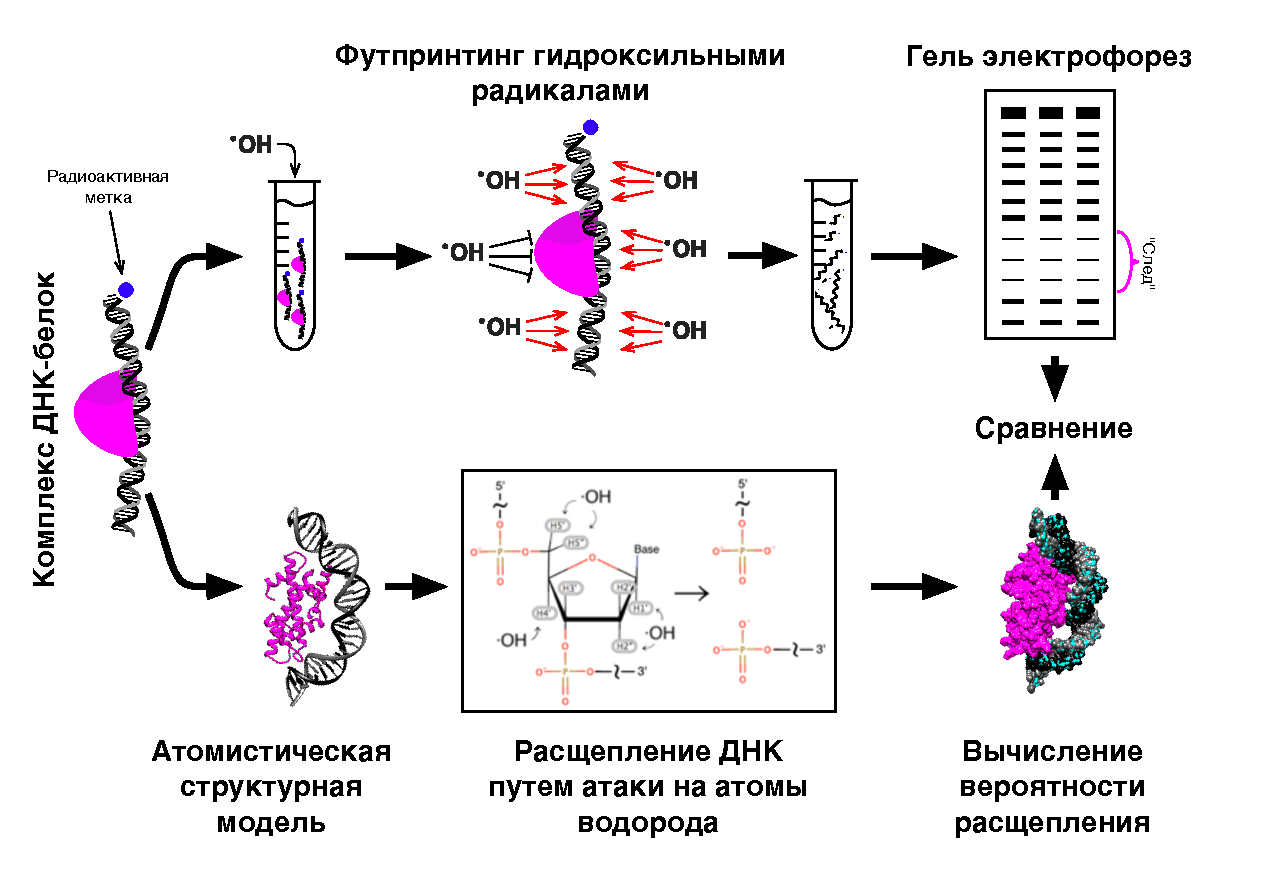
\includegraphics[width=\textwidth]{images/p5/part5_1_np/p5_1_f1.pdf}
    \caption[Футпринтинг комплексов ДНК-белок гидроксильными радикалами и структурная интерпретация экспериментальных данных.]{\textbf{Футпринтинг комплексов ДНК-белок гидроксильными радикалами и структурная интерпретация экспериментальных данных.} На схематической диаграмме изложены основные идеи использования HRF для выяснения структуры комплексов ДНК-белок. Вверху: комплексы ДНК-белок восстанавливаются на радиоактивно меченной ДНК и подвергаются расщеплению гидроксильными радикалами; гидроксильные радикалы расщепляют нити ДНК на участках, не защищенных белком, в режиме кинетики одиночных расщеплений (по одному разрезу на нить); Репертуар расщепленных фрагментов ДНК анализируется с помощью денатурирующего гель-электрофореза, и становятся очевидными положения в последовательности ДНК, защищенных белком. Внизу: атомистические структурные модели могут использоваться для прогнозирования профилей футпринтинга; частота расщепления зависит от доступности атомов водорода дезоксирибозы; сравнение предсказанных и экспериментальных результатов может быть использовано для уточнения или проверки структурных моделей.}
    \label{fig:p5_1_f1}
\end{figure}

\subsection{Разработка протокола}

    Теоретическая основа для количественной оценки экспериментальных данных футпринтинга гидроксильными радикалами была предложена ранее \cite{balasubramanian_dna_1998,shadle_quantitative_1997,das_safa_2005,bishop_map_2011}. Однако, столкнувшись с практической необходимостью структурной интерпретации данных HRF для комплексов ДНК-белок в наших недавних исследованиях \cite{shaytan_hydroxyl-radical_2017,xiao_molecular_2017}, мы поняли, что не существует простого протокола и программного обеспечения как для количественной оценки данных HRF, так и для анализа атомистической структуры. Ранее описанные подходы \cite{shadle_quantitative_1997,das_safa_2005}, которые использовались для количественной оценки результатов ПААГЭ или расчетов доступной для растворителя площади поверхности для анализа трехмерной структуры, утратили совместимость с современными компьютерными платформами или не имеют воспроизводимых примеров данных для их повторной реализации и проверки. Чтобы удовлетворить эту потребность, мы разработали свободно доступное программное обеспечение и здесь предоставляем пошаговые инструкции по его использованию.

    Мы представляем протокол и программный пакет HYDROID (HYDroxyl-Radical fOotprinting Interpretation for DNA). HYDROID обеспечивает: количественный анализ данных HRF с разрешением в один нуклеотид, оценку частот расщепления ДНК по кристаллическим структурам или атомистическим молекулярным моделям, сравнение и интеграцию этих подходов. HYDROID написан на Python и использует бесплатные кроссплатформенные компоненты ImageJ для анализа изображений \cite{schneider_nih_2012} и библиотеку FreeSASA для расчета площади поверхности \cite{mitternacht_freesasa_2016}. Кросс-платформенный и надежный характер структуры HYDROID поддерживается этими хорошо обслуживаемыми, регулярно обновляемыми и тщательно тестируемыми базовыми технологиями. Протокол HYDROID состоит из двух библиотек, HYDROIDexp (анализ и визуализация экспериментальных данных) и HYDROIDpred (анализ структуры) вместе с набором примеров и пошаговыми инструкциями. HYDROID количественно оценивает экспериментальные профили дорожек ПААГЭ с помощью аппроксимации данных с использованием различных функций и ограничений при проведении аппроксимации. Пакет оценивает теоретические профили частоты (интенсивности) расщепления ДНК на основе атомистических трехмерных структур путем вычисления доступной для растворителя площади поверхности атомов водорода дезоксирибозы. Чтобы ознакомиться с протоколом HYDROID, мы создали видеоурок по адресу \url{https://ncbi.github.io/HYDROID/docs/video.html}. Протокол успешно применялся в двух исследованиях \cite{shaytan_hydroxyl-radical_2017,xiao_molecular_2017}.

\subsection{Применение метода}

    HYDROID - это надежный, но гибкий инструмент для анализа и интерпретации экспериментов по футпринтингу ДНК. Он одновременно сочетает в себе функциональность для количественной оценки данных ПААГЭ продуктов футпринтинга (HYDROIDexp) и оценки профилей расщепления ДНК в ходе гидроксильного футпринтинга из экспериментальных структур или молекулярных моделей (HYDROIDpred).

    Ранее мы применили подход HYDROID для изучения центромерных нуклеосом дрожжей и их комплексов с белком CENP-C \cite{shaytan_hydroxyl-radical_2017,xiao_molecular_2017}. Высококачественный анализ экспериментальных данных HRF с помощью HYDROID позволил нам точно определить положение ДНК на октамере гистонов, построить атомистическую модель центромерной нуклеосомы, воссозданной на определенной последовательности ДНК, и идентифицировать сайты взаимодействий белка CENP-C с нуклеосомой.

    В этом разделе подход HYDROID был протестирован и подтвержден с использованием нескольких наборов экспериментальных данных по комплексам ДНК-белок. Мы проанализировали влияние различных параметров на производительность HYDROID и дали рекомендации относительно того, какие параметры следует использовать при анализе комплексов ДНК-белок. В разделе ``Экспериментальный дизайн'' представлены дополнительные сведения, соответствующие примеры и рекомендации.

    Основные функции модулей HYDROID можно легко адаптировать и использовать для более широкого спектра приложений. В частности, модуль HYDROIDexp сам по себе может применяться для анализа данных гель-электрофореза нуклеиновых кислот любого типа, обеспечивая точное количественное определение интенсивности полос. Алгоритмы аппроксимации полос, разработанные в HYDROIDexp, в целом могут быть адаптированы для анализа данных капиллярного электрофореза.

    Модуль HYDROIDpred в его нынешнем виде способен анализировать доступность атомов водорода рибозы/дезоксирибозы с использованием подхода вычисления поверхности доступной растворителю H-SASA для свободной ДНК или РНК или в комплексе с белками. Мы не проводили обширных испытаний подхода H-SASA для оценки профилей частоты расщепления в случаях, отличных от комплексов ДНК-белок. Однако другие исследования ранее показали, что оценка профилей H-SASA для определенных атомов водорода в нативной РНК или ДНК может быть аналогичным образом использована для оценки паттернов расщепления HRF \cite{bishop_map_2011,ingle_chemical_2014}. В таких случаях мы рекомендуем ознакомиться с указанными выше ссылками и указать в скрипте HYDROIDpred, какие атомы водорода следует учитывать для анализа. Учитывая важность метода HRF для анализа третичной структуры РНК и РНК-белковых комплексов \cite{costa_probing_2014,hampel_time-resolved_2001,nilsen_mapping_2014}, мы ожидаем, что части пакета HYDROID будут полезны для этой цели и потенциально могут быть включены в конвейеры предсказания структуры РНК \cite{ding_three-dimensional_2012,tian_rna_2016}.


\subsection{Сравнение с другими методами}

    Уникальной характеристикой HYDROID является интеграция количественной оценки экспериментальных данных HRF и анализа атомистической трехмерной структуры в одном пакете. Преимущества функциональности, предоставляемой отдельными компонентами HYDROID (HYDROIDexp и HYDROIDpred), обсуждаются ниже.
    
    Некоторые автономные программы были разработаны на протяжении многих лет для решения задач количественной оценки гелей в экспериментах HRF, такие как GelExplorer \cite{shadle_quantitative_1997} или SAFA \cite{das_safa_2005}. Однако одним препятствием при использовании этих программ в настоящее время является то, что они не обновлялись в течение некоторого времени и не совместимы с современными компьютерными системами. Дополнительные преимущества библиотеки HYDROIDexp включают возможность выбора гауссовой или лоренцевой формы полос и множество алгоритмов аппроксимации с ограничениями на вариации параметров. Библиотека HYDROIDexp также включает инструменты, совместимые с Python, для построения профилей вдоль последовательности ДНК. Это бесплатное программное обеспечение, которое можно повторно использовать в других проектах.

    Что касается теоретической оценки профилей расщепления ДНК из трехмерных структур, HYDROIDpred в настоящее время является единственным доступным решением. Он основан на вычислении доступности атомов водорода через библиотеку FreeSASA, которая является быстрой и бесплатной в использовании. HYDROIDprep расширяет ее, предоставляя для расчетов тщательно подобранные наборы атомных радиусов. Ранее сообщалось об альтернативном подходе (подход RADACK), который пытается учесть контролируемую диффузией природу реакции атаки гидроксильных радикалов и общую геометрию молекулы с помощью стохастического моделирования \cite{begusova_radack_2001}. Однако в настоящее время нет общедоступного программного обеспечения, реализующего подход RADACK.

\subsection{Преимущества и ограничения}

    Основным преимуществом HYDROID является его конструкция 2-в-1, предоставляющая пользователю возможность одновременно количественно оценивать экспериментальные данные HRF и сравнивать их с атомистическими структурными моделями комплекса белок-нуклеиновая кислота, если они доступны. Оба компонента HYDROID, реализующие эти функции, имеют свои преимущества. В частности, преимущества HYDROIDexp включают его кроссплатформенный характер (работает в Linux, Windows, MacOS) и одновременную реализацию ряда алгоритмов аппроксимации профиля HRF (формы полос Гаусса или Лоренца в сочетании с несколькими алгоритмами аппроксимации с ограничениями). Алгоритмы аппроксимации с ограничениями хорошо работают при деконволюции сигнала от частично перекрывающихся полос геля. Преимущества HYDROIDpred включают его бесплатную природу без каких-либо патентованных или лицензионных программных компонентов, а также тщательно отобранные и проверенные наборы параметров (радиус зонда, размеры атомов), которые можно использовать для получения значимых оценок профиля расщепления ДНК на основе молекулярных моделей. Алгоритм HYDROIDpred основан на оценке доступной для растворителя области атомов водорода дезоксирибозы. Этот подход не может напрямую объяснить кинетику диффузии гидроксильных радикалов (см. Раздел ``Схема эксперимента'' для дальнейшего обсуждения). Следовательно, следует проявлять осторожность при сравнении точных форм экспериментальных и теоретических профилей расщепления.

    Для подхода HYDROIDpred на вход должны быть поданы PDB-структуры с атомами водорода. Предлагаемый алгоритм добавления атомов водорода (шаг 23) в настоящее время работает только в Linux или Mac.


\subsection{Обзор протокола HYDROID}

    HYDROID состоит из протокола и программного пакета, написанного на языке Python, который вместе с другими компонентами (ImageJ и FreeSASA) представляет собой надежную основу для анализа и интерпретации экспериментальных данных футпринтинга гидроксильными радикалами ДНК-белковых комплексов. Протокол также может применяться для анализа комплексов РНК-белок, а также свободных молекул РНК/ДНК в растворе. Пакет программного обеспечения HYDROID можно легко установить в операционных системах Linux, Mac или Windows. Он состоит из двух дополнительных конвейеров (и соответствующих программных библиотек) HYDROIDexp и HYDROIDpred. Конвейер HYDROIDexp используется для анализа изображений геля ПААГЭ для получения значений частоты расщепления ДНК для каждой позиции на исследуемой последовательности ДНК (рис. \ref{fig:p5_1_f2}, вверху). Конвейер HYDROIDpred используется для выполнения теоретических расчетов частоты расщепления ДНК на основе трехмерной атомистической структуры или молекулярной модели комплекса ДНК-белок (рис. \ref{fig:p5_1_f2}, внизу). Расчеты частоты расщепления выполняются путем расчета доступной для растворителя площади поверхности атомов водорода дезоксирибозы (которые атакуются гидроксильными радикалами и вызывают расщепление ДНК) для каждого нуклеотида (профили H-SASA). Профили H-SASA позволяют оценить ожидаемую частоту расщепления ДНК. Сравнение и интегрирование экспериментальных и теоретических профилей можно в дальнейшем использовать для интерпретации экспериментальных данных и/или уточнения молекулярной модели. Основные программные функции, реализованные в пакете HYDROID, перечислены в таблице \ref{tab:p5_t1}. Они предназначены для запуска из сценария Python, а некоторые функции имеют интерактивный графический интерфейс пользователя. В пакете HYDROID полнофункциональные примеры данных HRF и анализа трехмерной структуры представлены в виде тщательно аннотированных скриптов Python. Эти примеры можно легко загрузить, и они служат в качестве изменяемых шаблонов для анализа пользовательских данных (см. ПРОЦЕДУРА и ОЖИДАЕМЫЕ РЕЗУЛЬТАТЫ). Ниже мы описываем методологию, лежащую в основе ключевых этапов структуры HYDROID. Видеоиллюстрации каждого этапа доступны по адресу \url{https://ncbi.github.io/HYDROID/docs/video.html}.

\subsection{Конвейер HYDROIDexp}
 Конвейер HYDROIDexp требует в качестве входных данных изображение геля ПААГЭ с дорожками для продуктов HRF одной из нитей ДНК и соседних дорожек с продуктами реакций секвенирования ДНК для той же цепи. Конвейер дает значения относительной частоты расщепления ДНК (также называемые значениями интенсивности расщепления ДНК) вдоль последовательности ДНК. Этот конвейер можно применять параллельно к нескольким образцам, которые были обработаны на одном и том же геле. Конвейер состоит из пяти этапов. См. Диаграмму рабочего процесса на рисунке \ref{fig:p5_1_f2}.


\begin{figure} [H]
    \centering
    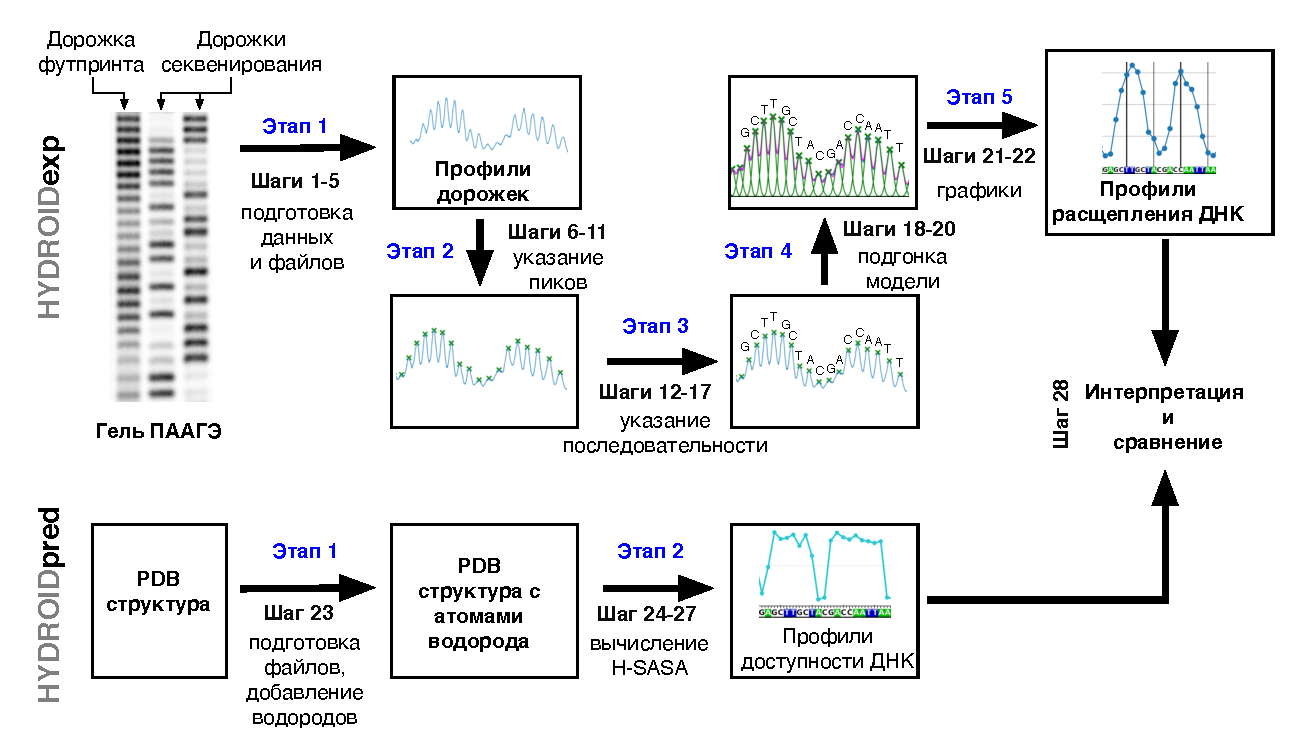
\includegraphics[width=\textwidth]{images/p5/part5_1_np/p5_1_f2.pdf}
    \caption[Конвейеры данных в HYDROID]{Конвейеры данных в HYDROID. Схематическая диаграмма для анализа экспериментальных данных по футпринтингу гидроксильными радикалами (вверху, HYDROIDexp). Теоретическая оценка профилей расщепления ДНК по молекулярным структурам (внизу, HYDROIDpred). Шаги и этапы процедуры аннотированы на схеме. Конвейер HYDROIDexp состоит из пяти этапов (отмечены синим цветом): этап 1 - профили дорожек в виде файлов данных извлекаются из изображения ПААГЭ, этап 2 - положения полос/пиков назначаются полуавтоматически на профилях дорожек, этап 3 - соответствие между полосами геля и последовательностью ДНК устанавливается, этап 4 - математическая модель подбирается для описания формы профиля дорожки с помощью функций Гаусса или Лоренца, этап 5 - интенсивности отдельных полос (частоты расщепления ДНК) извлекаются из модели. Конвейер HYDROIDpred состоит из двух этапов: этап 1 - загружается файл PDB интересующей системы и добавление атомов водорода к атомистической структуре при необходимости, этап 2 - профили доступности ДНК рассчитываются путем оценки доступной для растворителя области атомов водорода дезоксирибозы (H-SASA). Наконец, можно сравнить наборы теоретических и экспериментальных данных.}
    \label{fig:p5_1_f2}
\end{figure}



    \emph{Этап 1: Извлечение профилей дорожек геля}. Экспериментальные профили дорожек извлекаются из изображения геля. Экспериментальный профиль интенсивности полосы геля (профиль полосы) в дальнейшем определяется как массив значений интенсивности на изображении геля вдоль указанной полосы гель-электрофореза (в направлении миграции ДНК по гелю). Функции HYDROID считывают данные экспериментального профиля гелевой дорожки, сохраненные в виде столбцов чисел в текстовых файлах. Для получения ``цифровых'' экспериментальных профилей дорожек из изображений гелей ПААГЭ мы предлагаем использовать программное обеспечение ImageJ \cite{schneider_nih_2012} с плагином Bio-Formats \cite{linkert_metadata_2010} везде, где это необходимо для открытия файлов определенных форматов изображений гелей. 
    %Во вставке 2 приведены подробные инструкции по извлечению профилей полос в совместимом текстовом файле табличного формата из изображения СТРАНИЦЫ с помощью ImageJ. 
    Чтобы HYDROID мог считывать данные из сгенерированного файла, необходимо указать отдельный текстовый файл конфигурации, в котором указываются имена дорожек и соответствующие имена столбцов в сгенерированном файле.
    %(см. Блок 3 для более подробной информации о форматах входных файлов для HYDROIDexp. ).

    \emph{Этап 2: Назначение отдельных полос/пиков на геле}. Положение отдельных полос геля идентифицируется на профиле полосы геля с помощью полуавтоматического интерактивного алгоритма. Для деконволюции профиля полосы в набор вкладов от отдельных полос, сначала нужно знать количество и приблизительное расположение полос на профиле дорожки. Каждая полоса обычно соответствует локальному пику на профиле дорожки. Полуавтоматический интерактивный алгоритм, реализованный в
     функции \textit{assign\_peaks\_interactive} в HYDROID, открывает графическое окно и позволяет пользователю изменять параметры процедуры поиска пиков до тех пор, пока все необходимые пики не будут правильно идентифицированы по оценке пользователя. Алгоритм поиска пиков основан на библиотеке PeakUtils Python.
      Алгоритм регулируется двумя параметрами: относительной известностью пиков (параметр пикового порога - будут обнаружены только пики с амплитудой выше порога) и минимальным расстоянием между пиками. Алгоритм поиска пиков разделяет профиль полосы на несколько сегментов и позволяет пользователю выбирать минимальное расстояние между пиками для самого левого и самого правого сегментов (параметры \textit{min\_dist\_left} и \textit{min\_dist\_right}); значения в промежуточных сегментах затем выводятся с использованием линейной интерполяции. Если некоторые полосы перекрываются до такой степени, что пики не могут быть идентифицированы на профиле полосы или интенсивность полосы очень мала, в HYDROID реализована опция интерполяции пиков, чтобы попытаться вывести их положения из известных положений и расстояний между соседними группами, которые более заметны. Наконец, положения пиков можно указать вручную в файле конфигурации.

    \emph{Этап 3: Привязка пиков HRF к последовательности ДНК}. Каждую полосу на дорожке геля HRF (которая эквивалентна пику на профиле дорожки HRF) можно отнести к определенному положению в последовательности ДНК путем сравнения дорожек геля HRF с дорожками с продуктами реакций секвенирования ДНК для тех же ДНК. В HYDROID функция \textit{call\_peaks\_interactive} позволяет интерактивно строить профиль дорожки HRF вместе с профилями реакций секвенирования ДНК и последовательностью ДНК. Визуально сравнивая их с последовательностью ДНК, пользователь может указать местоположение любого одиночного пика на профиле и его соответствующее положение на последовательности ДНК. Это позволяет установить соответствие между всеми полосами и положениями в последовательности ДНК.

    \emph{Этап 4: Аппроксимация профилей интенсивности дорожек.} Математические модели, описывающие распределение интенсивности каждой полосы с помощью функций Гаусса или Лоренца, подгоняются к данным профиля полосы с помощью функции \textit{fit\_peaks}. Эта процедура позволяет вам провести деконволюцию необработанного экспериментального профиля HRF на вклады отдельных полос геля, тем самым должным образом принимая во внимание такие эффекты, как частичное перекрытие сигналов полос и неравномерная ширина полосы вдоль полосы геля 
    %(см. Вставку 4 для математических деталей алгоритма). 
    Известно, что эта процедура подвержена от переобучению, если на алгоритм подгонки не накладываются дополнительные ограничения \cite{takamoto_semi-automated_2004}. В HYDROID реализован ряд различных вариантов подгонки с ограничениями, перечисленных в Таблице \ref{tab:p5_t2}. См. Раздел ``Проблемы при экспериментальной количественной оценке профилей HRF'' для обсуждения дополнительных деталей.

    Чтобы оценить качество подгонки экспериментального профиля полосы с помощью модели, HYDROID предоставляет несколько критериев оценки: RMSD - среднеквадратичное отклонение между экспериментальными и прогнозируемыми значениями модели, относительное RMSD - вариация последнего, где отклонение в каждой точке выражается как часть экспериментального значения, и коэффициент корреляции Пирсона между экспериментальными и прогнозируемыми значениями.

    Значения частоты расщепления ДНК (общие площади под пиками на профиле дорожек) оценивают методом нелинейной аппроксимации методом наименьших квадратов. Для каждого пика площадь рассчитывается под сегментом кривой, который включает этот пик. Сегмент определяется серединами между положением данного пика (положением его максимума) и положением пиков его соседей слева и справа. Относительные различия в значениях прокси-площади, определенных для экспериментального профиля дорожки, по сравнению с профилем подобранной модели, используются как оценки неопределенности и называются ``относительными ошибками площади пика''. Максимальная относительная ошибка площади пика среди всех пиков, а также среднеквадратическое значение (``RMSD относительной площади пика'') вычисляются в HYDROID.
    
    \emph{Этап 5: Расчет частоты расщепления ДНК.} Частота расщепления ДНК для каждой позиции на ДНК вычисляется как площадь под гауссианой/лоренцевой кривой, описывающей соответствующую полосу. Значения профиля частоты расщепления ДНК отображаются вдоль последовательности ДНК.
    
    \subsection{Конвейер HYDROIDpred}
     Теоретический расчет профилей расщепления ДНК с помощью HYDROID основан на анализе трехмерных атомистических структур комплексов белок-ДНК и оценке доступности атомов водорода дезоксирибозы для гидроксильных радикалов. Трехмерные координаты можно получить с помощью рентгеновской кристаллографии или молекулярного моделирования (моделирование по гомологии, интегративное моделирование, докинг и т. д.). Доступная для растворителя площадь поверхности атомов водорода дезоксирибозы рассчитывается для каждого нуклеотида в молекуле ДНК структурного комплекса, что приводит к двум профилям H-SASA, по одному для каждой цепи (в случае, если протокол применяется к РНК, это приведет к одному профилю H-SASA). Он дает оценочные значения относительной частоты расщепления ДНК. Конвейер состоит из трех основных этапов.
    
    \textit{\emph{Этап 1:}Приготовление атомистической модели комплекса ДНК-белок с известными положениями атомов водорода.} Важным шагом является определение положений атомов водорода, если они отсутствуют в исходной структуре. Небольшие различия в положениях атомов водорода (например, разные параметры длины для связей C-X) могут повлиять на величину оцененных профилей (см. Подробное обсуждение в разделе ``Проблемы оценки теоретических частотных профилей расщепления ДНК из атомистических структур''). Программа REDUCE \cite{word_asparagine_1999} из пакета AmberTools 17 \cite{case_amber_nodate} с расстояниями связей X-H, полученными из  положений ядер атомов, может использоваться при добавлении атомов водорода в рентгеновские структуры.
    
    \emph{Этап 2:} \textit{Оценка теоретической частоты расщепления ДНК.} Теоретические профили частоты расщепления ДНК оцениваются путем расчета доступной для растворителя площади поверхности атомов водорода дезоксирибозы (профили H-SASA) с помощью функции get\_DNA\_H\_SASA, которая использует библиотеку FreeSASA \cite{mitternacht_freesasa_2016}. Алгоритм Ли-Ричардса используется \cite{lee_interpretation_1971} в FreeSASA с точностью до 200 срезов на атом по умолчанию. Для расчета SASA могут применяться другие радиусы зонда, по умолчанию 1,4\AA. HYDROID реализует три набора атомных радиусов для расчетов H-SASA: a) радиусы FreeSASA по умолчанию, б) значения радиусов из силового поля CHARMM36 \cite{best_optimization_2012} и в) значения радиусов из силового поля AMBER ff10 (parm10) \cite{case_amber_nodate}. Последние два получены из параметров rmin ван-дер-Ваальса (расстояние/радиус, при котором энергия Леннарда-Джонса имеет минимум) соответствующих силовых полей. Затем выполняется визуализация рассчитанных профилей (см. Визуализация и сравнение данных ниже).
    
    
    \subsection{Визуализация и сравнение данных}
    
    Для визуализации и сравнения профиля частоты расщепления ДНК HYDROID включает модуль построения графиков (\textit{plot\_prof\_on\_seq}) на основе библиотеки Matplotlib \cite{hunter_matplotlib_2007}. Этот модуль может одновременно строить несколько профилей вместе с последовательностью ДНК и позволяет использовать несколько методов нормализации (для приведения профилей к одному масштабу). Реализованы некоторые тривиальные методы нормализации, такие как деление каждого профиля на его максимальное значение (``every\_method'') или деление обоих профилей на их максимальное общее значение (``together\_method''). Кроме того, ``метод подгонки'' выполняет линейную регрессию без свободного члена между значениями профиля и изменяет их масштаб максимизируя взаимное максимальное соответствие. Использование линейной регрессии без свободного члена соответствует физическому требованию, согласно которому позиции, недоступные для расщепления, должны иметь нулевые значения на обоих профилях.

    Кроме того, мы реализовали метод моделирования профилей полос геля и изображений геля из профилей частоты расщепления (функция \textit{simulate\_gel}). Эта функция полезна для изучения ожидаемой формы профилей гелевых полос (и, следовательно, разрешения профиля в конкретной интересующей области ДНК) и планирования экспериментов. Модель подвижности ДНК Огстона используется для моделирования подвижности ДНК в геле \cite{slater_dna_2001}.
    


\begin{table}[h!]
    \centering
    \begin{tabularx}{\textwidth}{|X|X|}
        \hline
        \multicolumn{2}{|l|}{\textbf{Библиотека HYDROIDexp}} \\
        \hline
        assign\_peaks\_interactive & Предоставляет интерактивный интерфейс для полуавтоматического алгоритма, используемого для определения положения пиков на профилях гелевых дорожек.\\
        \hline
        call\_peaks\_interactive & Предоставляет интерактивный интерфейс для назначения индивидуальных пиков относительно положения последовательности ДНК.\\
        \hline
        fit\_peaks & Основная функция, которая подгоняет математическую модель профиля гелевой дорожки и оценивает интенсивность расщепления ДНК.\\
        \hline
        plot\_prof\_on\_seq & Строит любой профиль данных по последовательности ДНК и позволяет нормализовать и подгонять два или более профилей.\\
        \hline
        simulate\_gel & Имитирует форму профиля полосы геля и выводит изображение полосы геля на основе профиля H-SASA.\\
        \hline
        \multicolumn{2}{l|}{\textbf{Библиотека HYDROIDpred}} \\
        \hline
        get\_DNA\_H\_SASA & Оценивает теоретические профили расщепления ДНК (профили H-SASA) по структуре ДНК-белка.\\
        \hline
    \end{tabularx}
    \caption{Основные функции HYDROID и их описание.}
    \label{tab:p5_t1}
\end{table}



\begin{table}[h!]
    \centering
    \begin{tabularx}{\textwidth}{|X|X|}
        \hline
        Тип ограничения (аббревиатура) & Описание \\
        \hline
        dSIGMA>=0 & Ширина пика $\sigma$ не должна уменьшаться с увеличением D, положения пика (то есть от начала геля до конца). Это значительно повышает стабильность решения и предотвращает переобучение. \\
        \hline
        SIGMA<2*dD & Ширина пика $\sigma$ не может превышать удвоенное расстояние между данным пиком/полосой и последующим пиком (dD). Подразумевает автоматически ``dSIGMA> = 0''. \\
        \hline
        SIGMA=k*D+b & Ширина пика $\sigma$ линейно связана с положением пика (D). Это эффективно устанавливает линейную зависимость между шириной полосы и ее подвижностью. \\
        \hline
        log(SIGMA)=P2(log(M)) & Логарифм ширины пика $\sigma$ пропорционален логарифму числа нуклеотидов в ДНК, M, (или ее молекулярной массе) через полином второй степени. Оптимальные коэффициенты полинома определяются при подгонке: $\sigma_i = e^{a*(log M_i)^2 +b* log M_i +c}$) \\
        \hline
        SAFA & Ограничения, реализованные в программе SAFA \cite{das_safa_2005}, ширина пика связана с положением соседних пиков через $\sigma_i = \sigma_0 + k * \frac{D_{i + 1}-D_i}{2}$\\
        \hline
    \end{tabularx}
    \caption{Список ограничений при подгонке моделей, доступные в HYDROID.}
    \label{tab:p5_t2}
\end{table}


\subsection{Планирование экспериментов}
    
    \subsubsection{Метод HRF и интерпретация данных}
     В методе HRF используются гидроксильные радикалы, образованные в результате реакции Фентона или облучения, для расщепления цепей ДНК в доступных для растворителя участках \cite{jain_footprinting_2008-1}. Химический процесс, лежащий в основе, следующий: гидроксильный радикал атакует атомы водорода дезоксирибозы, что приводит к отщеплению водорода и последующему расщеплению основной цепи (рис. \ref{fig:p5_1_f1}). Основными продуктами этого химического расщепления являются две цепи, оканчивающиеся 3$^\prime$ и 5$^\prime$ фосфатами, которые примыкают к атакованному нуклеотиду в исходной цепи ДНК. Анализ продуктов расщепления ДНК обычно проводят с использованием денатурирующего электрофореза в полиакриламидном геле (ПААГЭ) предварительно радиоактивно/флуоресцентно меченой цепи (нитей) ДНК. Обычно рекомендуется радиоактивное мечение 5$^\prime$-конца ДНК \cite{jain_footprinting_2008-1}. В пределах кинетики единичного попадания (один разрез на цепь ДНК) доступность каждого нуклеотида для атаки гидроксильных радикалов должна быть пропорциональна интенсивности соответствующей полосы геля. Отнесение каждой полосы к определенному положению в последовательности ДНК является важным этапом и выполняется путем получения продуктов различных реакций секвенирования ДНК (таких, как реакции Максама-Гилберта) на соседних полосах геля (рис. \ref{fig:p5_1_f2}).
    
    Во время экспериментов по гидроксильному футпринтингу нуклеотид подвергается атаке гидроксильных радикалов, а затем разрушается, давая соответствующий фрагмент ДНК, который на один нуклеотид короче, чем предполагаемый фрагмент ДНК, оканчивающийся фактически атакованным нуклеотидом. Положение в последовательности ДНК, указанное пользователем на этом этапе, должно соответствовать нуклеотиду, который фактически подвергается атаке гидроксильных радикалов (и разрушается). Этот факт вместе с природой используемых реакций секвенирования ДНК следует учитывать при отнесении пика профиля HRF к положению в последовательности ДНК. Реакции секвенирования Максама-Гилберта удобны в этом отношении, поскольку они дают продукты, которые также на один нуклеотид короче, чем предполагаемые фрагменты ДНК, оканчивающиеся атакованным нуклеотидом \cite{maxam_new_1977}.
    
    Количественная оценка фактических частот расщепления ДНК требует измерения интенсивности отдельных полос из профилей интенсивности полос геля. Необходимо учитывать частичное перекрытие полос и изменение их ширины \cite{brahmasandra_mobility_2001}. Для определения общей интенсивности каждой полосы ранее была предложена математическая модель, которая использовалась для моделирования профиля интенсивности полос геля \cite{shadle_quantitative_1997}. При таком подходе интенсивность сигнала каждой полосы описывалась колоколообразной функцией, а результирующий профиль моделировался как сумма колоколообразных функций. К настоящему времени было предложено несколько функций моделирования, включая функции Гаусса, Лоренца \cite{shadle_quantitative_1997}, упрощенную интегрированную функцию Вейбулла \cite{bamidis_improved_2010} и более сложные функции \cite{greenbaum_construction_2007}. Хотя функция Гаусса является моделью по умолчанию для описания расширения полосы из-за свободной диффузии молекул, следует также учитывать некоторые другие факторы (например, электрическое поле, градиенты температуры, неоднородности геля и т. д.). В частности, методы радиографической детекции сигнала с геля могут изменять исходный сигнал, делая в некоторых случаях более подходящей модель функции Лоренца \cite{berg_appendix_1997}. По нашему опыту, данные, полученные для гелей с использованием современных установок, хорошо соответствуют функциям Гаусса. Более того, переобучение (overfitting) - обычная проблема для этих типов задач, и ее можно решить, наложив дополнительные ограничения на решение \cite{takamoto_semi-automated_2004}.
    
    Качество изображения геля, которое используется для извлечения профилей полос геля, является важной характеристикой, которая может повлиять на качество количественной оценки результатов HRF. Для получения хороших результатов ожидается, что в интересующей области будет отчетливо видна лестница из электрофоретических полос, представляющих продукты расщепления ДНК, отличающийся длинной в один нуклеотид. Однако протокол HYDROID также может быть успешным при деконволюции профилей дорожек в регионах, где некоторые полосы плохо видны или имеют значительное перекрытие. В этом случае пользователь должен иметь возможность указать количество ожидаемых диапазонов и их приблизительное расположение. С этой целью можно использовать места полос на других дорожках геля.
    
    Вычислительное структурное моделирование комплексов ДНК-белок можно направлять и проверять с помощью методов футпринтинга ДНК с высоким разрешением. Существует острая необходимость в программном решении для выполнения этих задач и объединения экспериментальных данных с трехмерными структурными моделями. Ранее Balasubramanian et al. провели детальное исследование интенсивности разрыва цепи ДНК при атаке на различные атомы водорода дезоксирибозы \cite{balasubramanian_dna_1998}. Они обнаружили, что атомы H5$^\prime$ и H5$^\prime$$^\prime$ обладают самой высокой реакционной способностью, за ними следуют H4$^\prime$, H3$^\prime$, H2$^\prime$ + H2$^\prime$$^\prime$ и H1$^\prime$. Более того, было обнаружено, что реакционная способность атомов водорода хорошо коррелирует с их доступной для растворителя площадью поверхности (SASA), которую можно оценить с помощью рентгеновских структур или предсказать с помощью структурных моделей. Это открытие является основой для теоретической оценки частот расщепления ДНК по атомистическим структурам в HYDROID. Однако, как мы обсудим далее, надежная оценка SASA для атомов водорода в комплексе ДНК-белок требует тщательного выбора параметров, таких как атомные радиусы, радиус сферы зонда и детали алгоритмов размещения атомов водорода.
    
    \subsubsection{Количественная обработка экспериментального профиля HRF}
    Количественная оценка экспериментальных профилей дорожек HRF выполняется в HYDROID путем деконволюции формы экспериментального профиля как суммы гауссовых (или лоренцевых) функций с центрами в положениях полос. Подгонка модели без ограничений обычно приводит к физически неправильным решениям (хотя и с лучшими характеристиками согласия), часто видны явные нарушения в положениях и ширине колоколообразных кривых, соответствующих отдельным полосам (верхняя панель рис. \ref{fig:p5_1_f3}В, а также результирующая частота расщепления ДНК (рис. \ref{fig:p5_1_f4}). Чтобы решить эту проблему, в HYDROID реализовано несколько ограничений в алгоритмах аппроксимации (Таблица \ref{tab:p5_t1}). Наиболее гибким является алгоритм ``dSIGMA> = 0'', который не позволяет ширине функций Гаусса уменьшаться при переходе от начала геля к его концу. Это основано на физическом предположении, что расширение полосы (более высокие коэффициенты дисперсии) увеличивается вместе с подвижностью ДНК в полосе. Это ограничение делает подобранное решение качественным в большинстве случаев, налагая только минимальные ограничения (рисунок \ref{fig:p5_1_f3}). Однако всегда рекомендуется визуальный осмотр полученного решения. Среди методов аппроксимации с ограничениями алгоритм ``dSIGMA> = 0'' обычно обеспечивает наилучшее соответствие, если судить по характеристикам качества аппроксимации. Другие алгоритмы ограничений также обеспечивают разумные решения со значениями RMSD относительной площади пика менее 2\% и почти идентичными результирующими профилями частоты расщепления ДНК.
    
    Анализ деконволюции профиля гелевых дорожек в HYDROID может быть выполнен с использованием функций Гаусса или Лоренца для аппроксимации распределения интенсивности полос. Некоторые предыдущие исследования показали, что Лоренциан может лучше соответствовать данным электрофореза ДНК \cite{shadle_quantitative_1997}. Для наборов экспериментальных данных, используемых в этом исследовании, функция Гаусса давала лучший результат, чем функция Лоренца, хотя различия в качестве аппроксимации не превышали 2\%, оцененные с помощью относительного среднеквадратичного отклонения. Однако профили интенсивности расщепления ДНК имели заметную разницу: при использовании лоренциана максимальные интенсивности расщепления имели тенденцию быть выше, а минимальные интенсивности расщепления были ниже, чем те, которые получены с использованием функции Гаусса. Этот эффект может быть объяснен медленным затуханием хвостов лоренцевского распределения, что заставляет пики с более высокой интенсивностью вносить больший вклад в амплитуду сигнала в соседних полосах с низкой интенсивностью.
    
    В профилях дорожек ПААГЭ геля иногда могут отсутствовать легко идентифицируемые максимумы для определенных полос. Это может произойти из-за шума, низкой интенсивности некоторых полос или перекрытия полос. Пока пользователь может определить количество и приблизительное положение этих полос, алгоритмы деконволюции HYDROID могут надежно их количественно оценить. Рисунок \ref{fig:p5_1_f3} иллюстрирует это для левой части профиля геля, где некоторые полосы перекрываются. Количественная оценка профилей, полученных электрофорезом одних и тех же продуктов реакции на двух разных гелях, дала почти идентичные результаты (неопубликованные наблюдения).
    
    
    \subsubsection{Оценка теоретических частотных профилей расщепления ДНК из атомистических структур}
    Следуя идеям, приведенным в \cite{balasubramanian_dna_1998} HYDROID оценивает теоретические профили частоты расщепления ДНК гидроксильными радикалами путем вычисления доступной для растворителя площади поверхности (SASA) атомов водорода дезоксирибозы (называемой профилями H-SASA). В общем, тот же метод можно применять для расчета доступной для растворителя площади поверхности атомов водорода рибозы РНК. Чтобы понять влияние различных параметров на форму профилей H-SASA, мы взяли структуру нуклеосомы в качестве примера и рассчитали профили H-SASA с различными наборами параметров: радиус зонда, наборы атомных радиусов, методы добавления атомов водорода, вклады от разных атомов водорода. Интерактивные графики профилей H-SASA, рассчитанных с различными параметрами, доступны по адресу  \url{https://ncbi.github.io/HYDROID/examples/example1/results/nucl_H-SASA.html}. Зависимость профилей H-SASA от радиуса зонда довольно проста: зонды меньшего размера могут различать более мелкие детали окклюзии ДНК белком, но делают профиль менее гладким и более зависимым от локальной геометрии взаимодействий ДНК-белок. Радиус зонда 1,4 \AA{} является обычным выбором, но расчет профилей H-SASA с различными размерами зонда может быть полезным для характеристики взаимодействий ДНК-белок в различных масштабах.
    
    Профили H-SASA довольно существенно зависят от выбора наборов атомных радиусов (FreeSASA vs CHARMM36 vs AMBER10) и от алгоритма, используемого для добавления атомов водорода (их положения в рентгеновских структурах обычно не разрешаются). Методологически последовательный подход требует генерирования положений атомов водорода с использованием параметров топологии из того же силового поля молекулярной механики, которое используется для оценки атомных радиусов. Как показано ранее, профили H-SASA чувствительны к небольшим колебаниям в геометрии остова ДНК как из-за неточностей рентгеновской структуры, так и из-за деталей конформации ДНК \cite{shaytan_hydroxyl-radical_2017}. Чтобы решить эту проблему, можно использовать моделирование молекулярной динамики (МД) для релаксации рентгеновских структур и анализа их динамики.  Основной вклад в H-SASA вносят значения площади, доступной для растворителя от атомов H5$^\prime$, H5$^\prime$$^\prime$ и H4$^\prime$ (рис. \ref{fig:p5_1_f5}A). Если H-SASA рассчитывается только для атомов H5$^\prime$, H5$^\prime$$^\prime$ и H4$^\prime$, соответствие между профилями, рассчитанными на основе MD и исходных рентгеновских структур, хорошее (рис. \ref{fig:p5_1_f5}Б). В частности, положения минимумов H-SASA (нуклеотиды ДНК, защищенные белком) подтверждаются между профилями (включая профили МД H-SASA, рассчитанные со всеми рассматриваемыми атомами водорода дезоксирибозы). Следовательно, при использовании рентгеновских структур без МД-релаксации рекомендуется расчет профилей H-SASA на основе только атомов H5$^\prime$, H5$^\prime$$^\prime$ и H4$^\prime$.
    
    Различия в форме экспериментальных и теоретических профилей расщепления ДНК можно объяснить двумя фактами. Во-первых, поскольку эксперименты с HRF проводятся в растворе, динамический характер конформации ДНК и взаимодействий между ДНК и белком могут привести к усреднению экспериментального профиля. Такие эффекты невозможно учесть теоретически, если не рассматривать и не анализировать динамический ансамбль структур. Во-вторых, из-за контролируемой диффузией природы реакции атаки гидроксильных радикалов, общая геометрия молекулы, включая ширину бороздок ДНК, также может модулировать вероятность атаки \cite{bishop_map_2011,begusova_radack_2001,spotheim-maurizot_radiation_2011}. Профили H-SASA могут лишь частично улавливать такие эффекты. Следовательно, при сравнении теоретических и экспериментальных профилей акцент следует делать на сравнении положений нуклеотидов, которые максимально защищены от атаки гидроксильными радикалами. Эффекты контролируемые диффузией отсутствуют для позиций ДНК, полностью защищенных белком.
    
    \subsection{Примеры данных}
    
    Протокол HYDROID использует два набора экспериментальных данных (названные ``Пример 1'' и ``Пример 2'', доступные  в репозитории GitHub), чтобы проиллюстрировать работу HYDROID. Пример 1 содержит данные HRF для центромерных нуклеосом \textit{S. cerevisiae}, восстановленных на последовательности ДНК 601TA с 3$^\prime$-концами, меченными радиоактивно, а пример 2 содержит данные HRF нуклеосом \textit{G. gallus}, восстановленных на последовательности ДНК 601 с 5$^\prime$-концами, меченными радиоактивно. Детали эксперимента для первого и второго наборов можно найти в ссылках \cite{shaytan_hydroxyl-radical_2017,xiao_molecular_2017} и \cite{morozov_using_2009} соответственно.

    Оба набора экспериментальных данных снабжены набором скриптов Python, которые образуют конвейер для анализа данных с использованием HYDROID и ожидаемых результирующих файлов.

    Пример 1 также предоставляет файлы с трехмерными координатами - молекулярную модель центромерной нуклеосомы дрожжей с последовательностью ДНК 601TA \cite{cloutier_dna_2005} (которая недоступна в PDB), которая была построена посредством моделирования по гомологии (с использованием Modeller \cite{sali_comparative_1993} и 3DNA \cite{lu_3dna_2008}). Последовательности гистонов были получены из HistoneDB2.0 \cite{draizen_histonedb_2016} и из соответствующей рентгеновской структуры нуклеосомы \textit{X. laevis} (PDB 3LZ0), как описано ранее \cite{shaytan_hydroxyl-radical_2017}. Программа REDUCE \cite{word_asparagine_1999} из пакета AmberTools 17 \cite{case_amber_nodate} использовалась для генерации положений атомов водорода с расстояниями связей X-H, полученных из положений ядер и электронных облаков. Кроме того, был использован подход молекулярной динамики. Используя команду VMD psfgen с силовым полем CHARMM36 \cite{best_optimization_2012}, гидратированные структуры были сгенерированы с последующим моделированием минимизации, релаксации и молекулярной динамики, как описано в наших более ранних исследованиях \cite{shaytan_hydroxyl-radical_2017}.
    
    \subsubsection{Опыт, необходимый для реализации протокола.} Пользователи должны быть знакомы с интерфейсом командной строки в Linux, Mac или Windows. Базовые знания языка сценариев Python были бы полезны для изменения простых сценариев Python с помощью текстового редактора. Для HYDROIDpred полезна часть понимания протокола формата PDB-файла.

    Оболочка графического пользовательского интерфейса (GUI) доступна для основных функций HYDROIDexp как дополнительный модуль по адресу \url{https://github.com/intbio/HYDROID_GUI} для тех пользователей, которые предпочли бы использовать GUI-интерфейс.
    
    
    
\begin{figure} [H]
    \centering
    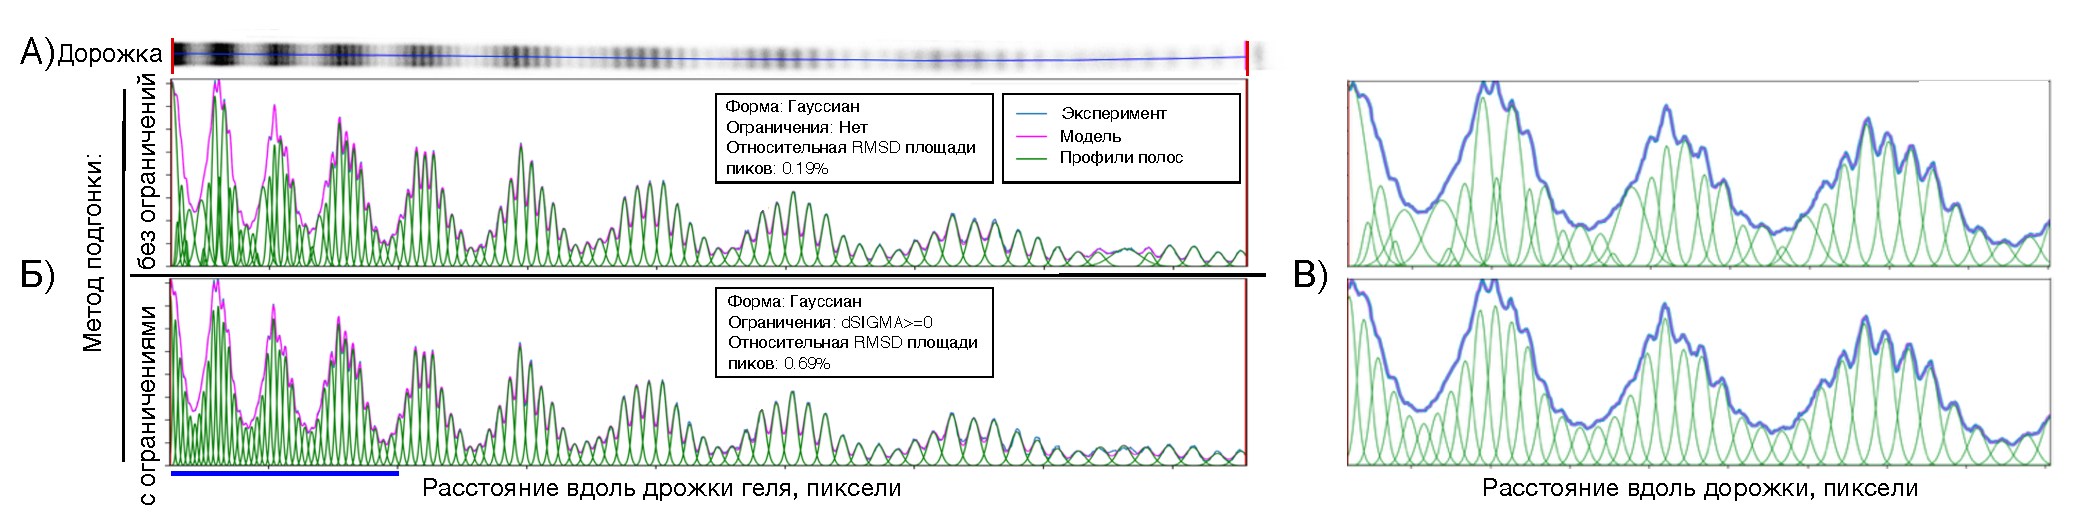
\includegraphics[width=\textwidth]{images/p5/part5_1_np/p5_1_f3.pdf}
    \caption[Количественная оценка изображения геля ПААГЭ путем подбора математической модели.]{Количественная оценка изображения геля ПААГЭ путем подбора математической модели. A) ПААГЭ изображение продуктов расщепления гидроксильными радикалами для одной цепи ДНК нуклеосомы. Направление миграции ДНК на изображении слева направо. Для получения этого изображения центромерные нуклеосомы  \textit{S. cerevisiae} воссоздали на хорошо позиционирующей последовательности ДНК 601TA с ДНК, радиоактивно меченной на 3'-конце. Расщепление ДНК, экстракция ДНК, ПААГЭ и получение радиоактивного сигнала выполнялись, как описано в \cite{shaytan_hydroxyl-radical_2017}. Б) Извлеченные профили дорожек аппроксимируются с помощью модели, которая представляет каждую полосу геля как функцию Гаусса, показаны результаты аппроксимации без и с ограничениями на параметры модели. Площадь под каждым гауссом представляет интенсивность полосы и, следовательно, частоту расщепления ДНК. В) Увеличенная версия графиков для левой части геля, выделенная синей линией на панели B. Неравномерности ширины и положения гауссианы для метода аппроксимации без ограничений хорошо видны. Экспериментальные и модельные кривые невозможно различить, потому что они почти перекрываются. Ось Y на графиках представляет значения интенсивности профиля.}
    \label{fig:p5_1_f3}
\end{figure}
    
    
    \subsection{Материалы}
    \subsubsection{Оборудование и данные}
    
    \textbullet \ Компьютер, работающий в среде Linux, Mac или Windows.
    \textbullet \ ПААГЭ изображения продуктов реакции HRF и продуктов реакции секвенирования ДНК (обычно получаемые с помощью фосфоимаджера, если фрагменты ДНК радиоактивно помечены). Файлы изображений должны иметь достаточно хорошее разрешение, чтобы в интересующей области расстояние между полосами было больше 10 пикселей. Формат файла изображения должен быть одним из тех, которые может читать ImageJ как таковой или через плагин BioFormats.
    \textbullet \ (Необязательно) 3D-атомистические структуры или молекулярные модели исследуемого комплекса ДНК-белок.
    
 
    \subsubsection{Скачивание примеров}

    Пакет HYDROID поставляется с набором примеров (шаблонов протоколов), доступных по ссылке \url{https://github.com/ncbi/HYDROID/tree/master/examples}. 
    
    \subsection{Описание протокола}
    
    ВАЖНО Перед выполнением процедуры убедитесь, что HYDROID и сопутствующие программные инструменты установлены.
    
    \subsubsection{Количественная оценка изображений HRF ПААГЭ (конвейер и библиотека HYDROIDexp)}
    
    
    
    1. \emph{Извлечение профилей полос из файлов изображений ПААГЭ и подготовка файлов данных для HYDROID.} Чтобы извлечь профиль полосы из изображения используйте программное обеспечение ImageJ.  Сохраните файл изображения с линиями, обозначающими диапазоны извлеченных данных, для дальнейшего использования.
    
    2. Загрузите образцы проектов анализа HRF, поставляемые с HYDROID.  Если ДНК в экспериментах с HRF была помечена на 3$^\prime$-конце, используйте пример 1; если ДНК в экспериментах с HRF была помечена на 5$^\prime$-конце, используйте пример 2. Папка примера проекта содержит сценарии Python для каждого этапа конвейера и папку данных с несколькими файлами данных, которые будут использоваться на следующих этапах.
    
    3. Замените файл \textsc{data/lane\_profiles.xls} файлом данных профилей полос, извлеченным из изображения ПААГЭ на шаге 1.
    
    4. Измените файл \textsc{data/lane\_config.csv}, чтобы указать, какие столбцы из файла \textsc{data/lane\_profiles.xls}  следует анализировать HYDROID, и укажите понятные человеку идентификаторы. На этом этапе для всех остальных параметров должно быть установлено значение NaN (используйте верхнюю строку исходного файла в качестве шаблона).

    5. Укажите исследуемую последовательность ДНК в файле \textsc{data/DNA\_seq.fasta}. 
    
    

    
    
    6. \emph{Определение положений пиков (местоположений электрофоретических полос) на профилях дорожек геля с помощью полуавтоматического интерактивного алгоритма.} Откройте сценарий \textsc{exp\_s2\_assign\_peaks.py}  в текстовом редакторе и измените переменную lane\_names (в строках 37–38), чтобы включить в нее имена полос из файла \textsc{data/lane\_config.csv} , которые следует проанализировать.

\emph{ВАЖНО:} Идентификация положений пиков в конечном итоге требуется только для дорожек с данными HRF, но ее можно использовать для изучения профилей дорожек секвенирования ДНК с помощью той же процедуры.

    7. Запустите сценарий с помощью следующей команды в терминале:
    \textsc{> Python exp\_s2\_assign\_peaks.py}
    Для каждой дорожки, указанной в Шаге 6, откроется интерактивное окно, показывающее график профиля дорожки и позволяющее настроить параметры алгоритма идентификации пиков, а также ряд дополнительных параметров.

    ВАЖНЫЙ ШАГ: Интерактивные окна открываются одно за другим. Пожалуйста, закройте каждое окно, чтобы перейти к следующему.
    
    8. Цели следующих шагов - указать диапазон данных для анализа и выделить каждый пик (полосу) в этом диапазоне звездочкой. Используйте интерактивные ползунки, чтобы указать диапазон значений профиля HRF, который будет анализироваться в дальнейшем (параметры \textsc{leftlim} и \textsc{rightlim}).

    9. Настройте \textsc{пиковый порог} (регулирует чувствительность алгоритма к величине пиков), \textsc{min\_dist\_left} (регулирует минимально допустимое расстояние между пиками в левой части диапазона данных), \textsc{min\_dist\_right} (регулирует минимально допустимое расстояние между пиками справа от диапазона данных), \textsc{baseline} (вычитает линейную базовую линию из данных перед попыткой идентифицировать пики) и \textsc{Segments} (устанавливает количество сегментов для разделения диапазона данных для интерполяции минимально необходимого расстояния между пиками) до тех пор, пока каждый пик (диапазон) не будет выделен только одной звездочкой.
        ВАЖНЫЙ ШАГ: В пределах анализируемого диапазона данных каждое местоположение полосы должно быть выделено только одной звездочкой. В противном случае последующий анализ будет некорректным.
        КРИТИЧЕСКИЙ ШАГ: Иногда интенсивность полос очень мала, данные зашумлены или полосы подходят так близко друг к другу, что на профиле полосы не видно локальных максимумов, представляющих полосу. Алгоритм деконволюции может работать хорошо в таких случаях, если ожидаемое положение полосы отмечено звездочкой. Последнее может быть достигнуто путем включения переключателя \textsc{Interpolate} в интерактивном окне. Алгоритм попытается угадать положения полос, которые не представлены определенным пиком на профиле HRF. Кроме того, положение полос можно указать вручную в файле \textsc{data/lane\_config.csv}. Для этого их местоположение можно ввести в столбец \textsc{addpeaks} файла.
    
    10. (Необязательно) Параметр \textsc{alignpos} позволяет указать положение любого пика, который будет использоваться на следующем этапе для выравнивания профиля HRF с профилями секвенирования ДНК для задания последовательности ДНК. Обычно это может быть заметный пик на конце геля, который однозначно идентифицируется как полоса, представляющая продукт ДНК одинаковой длины на дорожках HRF и секвенирования ДНК.

    11. Нажмите кнопку Сохранить. Данные будут записаны в файл \textsc{data/lane\_config.csv}. Повторите процедуру для других профилей полос.
    

    12.     \emph{Задание последовательности ДНК на профиле дорожки HRF.}  Откройте сценарий \textsc{exp\_s3\_call\_peaks.py} в текстовом редакторе и измените список \textsc{lane\_sets}, включив в него имена дорожек HRF (\textsc{footprinting\_profile}) вместе с именами соответствующих профилей секвенирования ДНК (\textsc{helper\_profiles}) из файла \textsc{data/lane\_config.csv}.

    КРИТИЧНЫЙ ШАГ: Обязательно укажите правильный конец маркировки ДНК в переменной \textsc{метки} (начиная со строки 35). Убедитесь, что последовательность ДНК, предоставленная для каждого профиля дорожки HRF (переменная \textsc{seq}), соответствует конкретной последовательности ДНК цепи ДНК, которая использовалась в эксперименте (записана в обозначениях 5 $^\prime$-> 3$^\prime$).
    
    13. Запустите сценарий с помощью следующей команды:
    \textsc{> Python exp\_s3\_call\_peaks.py}
    Для каждого профиля дорожки HRF, указанного на шаге 12, откроется интерактивное окно, где он будет нанесен на график вместе с соответствующими профилями секвенирования ДНК. Также будет показана последовательность исследуемой цепи ДНК.

    14. Цель следующих шагов 14-17 состоит в том, чтобы вручную сопоставить любой пик на профиле HRF с соответствующим положением в последовательности ДНК, просматривая профили секвенирования ДНК, нанесенные на тот же график. При необходимости используйте ползунки \textsc{alignpos}, чтобы выровнять профили секвенирования ДНК друг с другом и профилем HRF.
    
    15. Используйте ползунок \textsc{последовательности}, чтобы выбрать позицию в последовательности ДНК (выбранная позиция будет выделена заглавной буквой).

    16. Используйте ползунок \textsc{seqpeak}, чтобы навести стрелку на пик профиля дорожки HRF, соответствующий положению в последовательности ДНК, идентифицированной на предыдущем шаге.
    
  КРИТИЧЕСКИЙ ШАГ: Пользователь должен понимать природу выбранной реакции секвенирования ДНК и ее продуктов, чтобы правильно выполнить этот шаг (см. Дизайн эксперимента).

    17. Нажмите кнопку Сохранить. Данные будут записаны в файл \textsc{data/lane\_config.csv}. Повторите процедуру для других профилей дорожек HRF.


    
    
    
    18.     \emph{Подбор модели к профилю дорожки HRF для количественной оценки частот расщепления ДНК.} Откройте скрипт \textsc{exp\_s4\_fit\_model.py} в текстовом редакторе и измените список \textsc{lane\_data}, включив в него имена дорожек HRF, которые будут подвергаться количественной оценке. Параметры функции \textsc{fit\_peaks} также можно изменить для настройки результатов: для параметра \textsc{peaktype} можно задать значение Гаусса или Лоренца в зависимости от желаемой модели полосы, \textsc{Fit\_constraint} может принимать одно из значений, указанных в Таблице \ref{tab:p5_t2}, \textsc{maxfev} управляет максимальным количеством шагов оптимизации, установите меньшее количество, чтобы получить быстрые предварительные результаты.

    19. Запустите сценарий с помощью следующей команды:
    \textsc{> Python exp\_s4\_fit\_model.py}

    20. Скрипт выведет интерактивные графические окна с графиками результатов подгонки (Рисунок \ref{fig:p5_1_f3}Б). Результаты будут автоматически сохранены в CSV-файл, указанный в скрипте (\textsc{results/LANE\_NAME\_fitted\_intensities.csv}). Скрипт будет запускаться последовательно для всех профилей дорожек.
    ВАЖНЫЙ ШАГ. Пользователь должен изучить полученные графики (при необходимости увеличить масштаб, используя кнопку масштабирования) и убедиться, что в результатах подгонки нет отклонений, подобных тем, которые показаны на верхних панелях рисунков \ref{fig:p5_1_f3}Б, \ref{fig:p5_1_f3}В. 
    


    21.     \emph{Построение графика частоты расщепления вдоль последовательности ДНК.}
        HYDROID предоставляет настраиваемую функцию \textsc{plot\_prof\_on\_seq}, которую можно использовать для построения графиков профилей данных поверх последовательности ДНК (рисунок \ref{fig:p5_1_f4}). Откройте сценарий \textsc{exp\_s5\_plot\_cl\_freq.py} в текстовом редакторе и измените список \textsc{lane\_data} (рядом со строкой 28), включив в него имена файлов, содержащих результаты количественной оценки из шага 20. Также можно указать заголовок графика и имя выходного файла (строки 40-43).

    22. Запустите сценарий с помощью следующей команды:
        \textsc{> python exp\_s5\_plot\_cl\_freq.py}
        Откроются интерактивные окна с графиками, и графики будут сохранены в \textsc{results/LANE\_NAME\_fitted\_intensities.png}.
    
    \subsubsection{Прогнозирование интенсивности расщепления на основе атомистических трехмерных структур (конвейер и библиотека HYDROIDpred).}
    
    23.     \emph{Подготовка файла PDB с трехмерной структурой комплекса ДНК-белок}. Файл PDB, представляющий вашу экспериментальную систему, может быть доступен в базе данных PDB (www.pdb.org) или быть продуктом молекулярного моделирования. Поскольку в структурах PDB, полученных с помощью рентгеновских лучей, часто отсутствуют атомы водорода, вы можете использовать следующую команду для добавления атомов водорода:
    \textsc{> reduce -NUClear file.pdb> file\_H.pdb}
    где file.pdb - это имя исходного файла PDB.
    
    
    Полученный PDB-файл должен быть сохранен в подкаталоге \textsc{data/structure}.

    
    
    
    24. \emph{Запустите расчеты SASA, чтобы оценить профили частоты расщепления ДНК.} Откройте скрипт \textsc{pred\_s2\_calc\_H-SASA.py} в текстовом редакторе и измените список \textsc{prof\_data}, включив в него имя (имена) файла(ов) структуры PDB, идентификатор PDB цепи, которая представляет рассматриваемую нить ДНК, остатки. Параметр должен указывать диапазон номеров остатков из PDB-файла, который будет анализироваться, параметр \textsc{seq} должен указывать последовательность ДНК исследуемой цепи. Параметр \textsc{Hcontrib}  представляет собой список из семи чисел, который определяет вес вклада каждого отдельного атома водорода дезоксирибозы в следующем порядке [H1' H2' H2'' H3' H4'H5' H5'']. Для рентгеновских структур с низким и средним разрешением (выше 2,5-3\AA) предлагается учитывать только вклады атомов H4', H5' и H5''.

    25. Запустите сценарий с помощью следующей команды:
            \textsc{> python pred\_s2\_calc\_H-SASA.py}
        Предполагаемые профили расщепления ДНК будут сохранены в файлах CSV \textsc{results/PROF\_NAME\_H-SASA.csv}, где PROF\_NAME - имя, указанное ранее в списке \textsc{prof\_data}.


    26. \emph{Построение расчетных частот расщепления ДНК вдоль последовательности ДНК} Откройте сценарий \textsc{pred\_s3\_plot\_H-SASA.py} в текстовом редакторе и измените список \textsc{lane\_data}, включив в него имя файла CSV с предполагаемым профилем, последовательность ДНК исследуемой цепи и имя выходного файла.
    
    27. Запустите сценарий с помощью следующей команды:
            \textsc{> python pred\_s3\_plot\_H-SASA.py}
        Откроются интерактивные окна с графиками, дополнительно графики будут сохранены в виде файлов PNG.

    
    \subsubsection{Сравнение данных, полученных из конвейеров HYDROIDexp и HYDROIDprep}
    
    28. Данные из файлов CSV, полученные на этапах 20 (экспериментальные профили) и 27 (теоретические профили), можно открыть, нанести на график и сравнить с помощью любого программного обеспечения для построения графиков, предпочитаемого пользователем (например, MS Excel). CSV-файл, созданный конвейером HYDROIDexp (см., Например, \textsc{results/scCSE4\_601TA\_BS\_fitted\_intensities.csv} в примере 1), имеет столбцы с именами \textit{Site} и \textit{Intensity}, соответствующие положению последовательности ДНК и количественной оценке интенсивности/частоты расщепления ДНК, соответственно. CSV-файл, созданный конвейером HYDROIDpred (см., Например, \textsc{results/scCSE4\_601TA\_BS\_H-SASA.csv} в примере 1), имеет столбцы с именами \textit{Site} и \textit{H-SASA}, соответствующие положению последовательности ДНК и теоретически оцененной вероятности расщепления ДНК, соответственно.
    Для тех, кто обладает продвинутыми навыками в языке Python, мы предоставляем примеры для обработки и построения результатов примера 1 в файле \textsc{com\_plot\_ex\_vs\_pred.py}.
    
    \subsubsection{Временные затраты}

    Время, необходимое для протокола, зависит от количества экспериментальных образцов для анализа и знакомства пользователя с инструментами командной строки и языком сценариев Python. Оценки для изображения ПААГЭ геля с двумя дорожками HRF и четырьмя дорожками секвенирования ДНК на основе Примера 1 представлены ниже:

    Шаг 1. Обработка файла изображения с помощью Fiji ImageJ: 30 мин.

    Шаги 2-11, Определение положения пиков (расположение электрофоретических полос): 30 мин.

    Шаги 12-17, определение последовательности ДНК на профиле дорожки HRF: 30 мин.

    Шаги 18-20, Подгонка модели к профилю дорожки HRF: 30 мин.

    Шаги 21-22, извлечение и нанесение на график частот расщепления вдоль последовательности ДНК: 10 мин.

    Шаг 23. Подготовка файла PDB с трехмерной структурой комплекса ДНК-белок: 15 мин.

    Шаги 24-25, Настройка и выполнение расчетов SASA для оценки профилей частоты расщепления ДНК: 20 мин.

    Шаги 26-27, нанесение на график расчетных частот расщепления ДНК вдоль последовательности ДНК: 5 мин.
    
% \begin{table}[h!]
%     \centering
%     \begin{tabularx}{\textwidth}{|X|X|X|X|}
%         Шаги & Проблема & Возможная причина & Решение \\
%          \hline
%         Шаг 1 & В Fiji ImageJ изображение геля отображается в негативных цветах. & Таблица поиска настроена неправильно. & Нажмите Изображение-> Таблицы поиска-> Инвертировать LUT \\
%          \hline
%         Шаг 9 & Полуавтоматический алгоритм не может определить все необходимые местоположения диапазонов в профиле HRF. & Данные слишком зашумлены или величина пиков очень мала. & 1) Попробуйте настроить параметры так, чтобы четко идентифицировались только хорошо разрешенные пики. Нажмите на переключатель Interpolate, чтобы угадать недостающие позиции.
% 2) Если предыдущий вариант не решает проблему: запишите позиции полос, которые все еще отсутствуют, поместив указатель мыши в эти места. См. Инструкцию в файле \textsc{lane\_config.csv}  о том, как указать эти местоположения вручную в столбце \textsc{addpeaks}.\\
%          \hline
%         Шаг 20 & На полученном графике отдельные гауссианы, описывающие полосы на конце геля, слишком широки, чтобы представлять физически правдоподобное решение. & Произошла переобучение. & Используйте более строгий параметр ограничения подгонки, например, ``SIGMA=k*D+b''. \\
%          \hline
%         Шаг 27 & Теоретические профили расщепления ДНК выглядят шумно & Небольшие неровности трехмерной структуры могут повлиять на доступность атома водорода дезоксирибозы. & Используйте только вклады атомов водорода дезоксирибозы H4$^\prime$, H5$^\prime$ и H5$^\prime$$^\prime$ для оценки профиля расщепления. Установите для параметра \textsc{Hcontrib} значение $[0,0,0,0,1,1,1]$ \\
%          \hline
%     \end{tabularx}
%     \caption{Таблица поиска и устранения неисправностей.}
%     \label{tab:p5_ttrouble}
% \end{table}
    
    \subsection{Ожидаемые результаты}
    
    \subsubsection{Пример из практики: ДНК-белковые взаимодействия в нуклеосомах}
    
    В качестве примера применения HYDROID к системам ДНК-белок мы проанализировали и интерпретировали эксперименты HRF для нескольких нуклеосом, поскольку они представляют собой одну из самых сложных систем для изучения и демонстрируют периодические взаимодействия ДНК-белок. Были получены два независимых набора экспериментальных данных из разных лабораторий: а) HRF нуклеосом, восстановленных на 601 хорошо позиционирующей последовательности \cite{lowary_new_1998} с использованием гистонов из эритроцитов \textit{G. gallus}, б) HRF нуклеосом, восстановленных на аналогичной хорошо позиционирующей последовательности 601TA \cite{cloutier_dna_2005} с использованием рекомбинантных гистонов центромерных нуклеосом \textit{S. cerevisiae} \cite{shaytan_hydroxyl-radical_2017}. В двух независимых наборах данных также использовались разные методы маркировки ДНК: в первом случае был помечен 5$^\prime$-конец, а во втором - 3$^\prime$-конец.
    
    Результаты анализа этих экспериментов, а также сравнения с теоретическими профилями H-SASA представлены на рисунке \ref{fig:p5_1_f6}. Известно, что ДНК в нуклеосоме хорошо расположена в случае последовательности 601/601TA и намотана вокруг октамера гистона в сверхспиральной форме (рис. \ref{fig:p5_1_f6}А) интенсивности расщепления ДНК, как было ранее показано, очень похожи для верхней и нижней цепей из-за псевдосимметрии нуклеосомы \cite{shaytan_hydroxyl-radical_2017}. Профили расщепления ДНК отражают периодичность нуклеосомной ДНК 10-11 п.н., когда она вращается вокруг поверхности октамера гистонов (рис. \ref{fig:p5_1_f6}Б). Два экспериментальных профиля, полученные с использованием разной маркировки концов, хорошо совпадают, но отличаются в некоторых аспектах. Это может отражать воспроизводимость, которую можно ожидать от анализа HRF, выполненного с использованием различных протоколов. Ключевой характеристикой является положение минимумов и максимумов, в то время как точная величина расщепления ДНК может зависеть от экспериментальных условий, наличия частично собранных нуклеосомных состояний \cite{rychkov_partially_2017}, динамики ДНК и белков \cite{eslami-mossallam_nucleosome_2016}. Положения минимумов и максимумов совпадают с точностью до 1 нуклеотида между профилями (Рисунок \ref{fig:p5_1_f6}Б). Для ДНК, меченной 3$^\prime$-концом, в большинстве случаев минимумы смещены на одну пару оснований в сторону 5$^\prime$-конца ДНК по сравнению с экспериментом с ДНК, меченной по 5$^\prime$-концу. Возможное объяснение этой тонкой разницы заключается в том, что во время расщепления гидроксильных радикалов помимо основных продуктов с концевыми 5$^\prime$- и 3$^\prime$-фосфатами образуются другие второстепенные продукты. В частности, на 5$^\prime$-конце может быть образована цепь, оканчивающаяся 5$^\prime$-альдегидной группой \cite{balasubramanian_dna_1998}. Она на один нуклеотид длиннее цепи с 5'-фосфатным концом, в ней отсутствует отрицательный заряд фосфатной группы и его подвижность в геле на 2–3 нуклеотида ниже, чем у обычного продукта \cite{kappen_deoxyribonucleic_1983}. На 3$^\prime$-конце сайта расщепления второстепенным продуктом является 3$^\prime$-фосфогликолят, который, как известно, менее распространен и мигрирует близко к обычному продукту \cite{balasubramanian_dna_1998}. Таким образом, обычно рекомендуется мечение 5$^\prime$-конца ДНК.
    
    Пример сравнения теоретических профилей расщепления ДНК, извлеченных из структурной модели, и экспериментальных данных HRF показан на рисунке \ref{fig:p5_1_f6}В. Положения минимумов экспериментального и теоретического профилей совпадают с точностью до 1 нуклеотида. Форма теоретического профиля менее плавная, чем у экспериментального, что отражает ограничения теоретической модели. Более гладкая форма экспериментальных профилей, вероятно, связана с динамикой структур в растворе, а также с кинетическими эффектами, связанными с диффузией гидроксильных радикалов. Интерактивные веб-графики, сравнивающие профили H-SASA, полученные с разными параметрами, доступны в репозитории GitHub по ссылке \url{https://ncbi.github.io/HYDROID/examples/example1/results/nucl_H-SASAvsEXP_BS.html.} 
    
    
\begin{figure} [H]
    \centering
    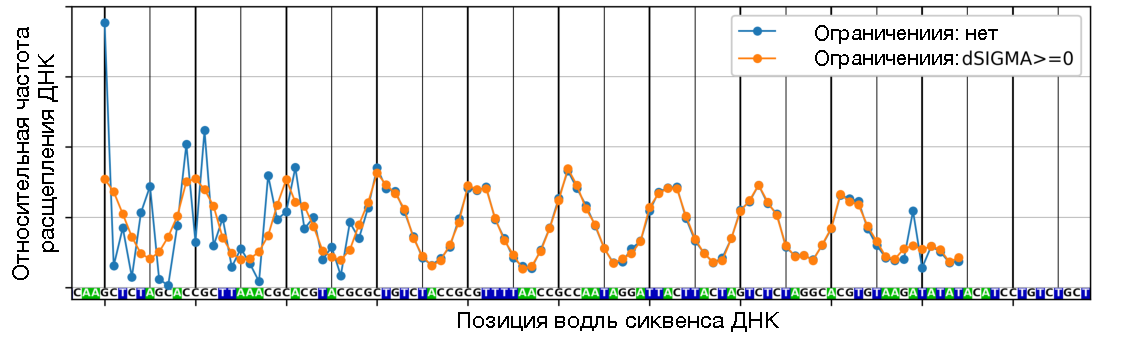
\includegraphics[width=\textwidth]{images/p5/part5_1_np/p5_1_f4.pdf}
    \caption[Профили частоты расщепления ДНК, извлеченные из экспериментов по гидроксильному футпринтингу.]{\textbf{Профили частоты расщепления ДНК, извлеченные из экспериментов по гидроксильному футпринтингу.} В соответствии с нашей методологией количественной оценки данных HRF кривая профиля полосы на рисунке \ref{fig:p5_1_f3}B была построена с помощью комбинации функций Гаусса. Области этих индивидуальных функций Гаусса представляют собой интенсивности отдельных полос и, следовательно, значения частоты расщепления ДНК. Эти количественные значения частоты расщепления ДНК представлены здесь как для аппроксимации с и без органичней на параметры модели. Соответствие между последовательностью ДНК и профилем HRF было идентифицировано с использованием продуктов реакций секвенирования Максама-Гилберта. Видны отклонения в значениях, полученные в результате аппроксимации без ограничений на параметры модели.}
    \label{fig:p5_1_f4}
\end{figure}
    
\begin{figure} [H]
    \centering
    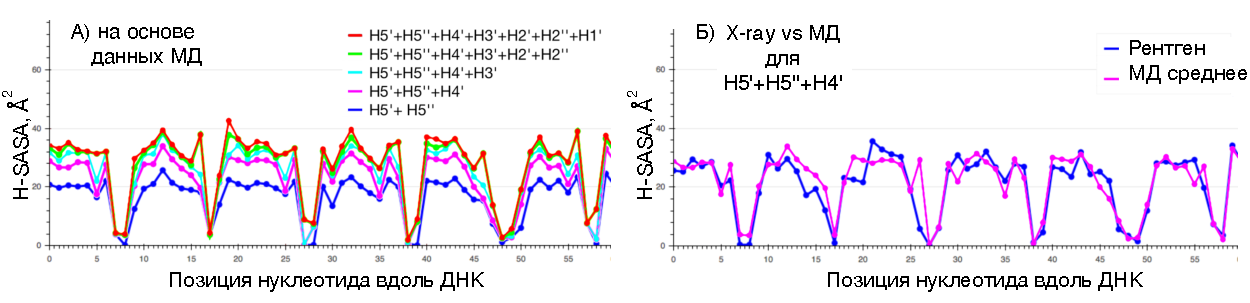
\includegraphics[width=\textwidth]{images/p5/part5_1_np/p5_1_f5.pdf}
    \caption[Профили H-SASA для ДНК в нуклеосомах]{Профили H-SASA для ДНК в нуклеосомах. A) Профили H-SASA (доступная для растворителя площадь поверхности атомов водорода дезоксирибозы) рассчитываются с использованием вкладов различных атомов водорода дезоксирибозы для каждого нуклеотида вдоль последовательности ДНК, начиная с центра нуклеосомы. Профили были рассчитаны путем усреднения более 50 снимков из МД моделирования с интервалом в 1 нс. Б) Сравнение профилей H-SASA (на основе атомов H5$^\prime$, H5$^\prime$$^\prime$ и H4$^\prime$), рассчитанныt на основе рентгеновской структуры (с атомами водорода, добавленными через программу REDUCE) и траектории МД. Если доступны только атомы H5$^\prime$, H5$^\prime$$^\prime$ и H4$^\prime$, профили не сильно различаются, и для надежной оценки профиля можно использовать рентгеновские структуры.}
    \label{fig:p5_1_f5}
\end{figure}
    
\begin{figure} [H]
    \centering
    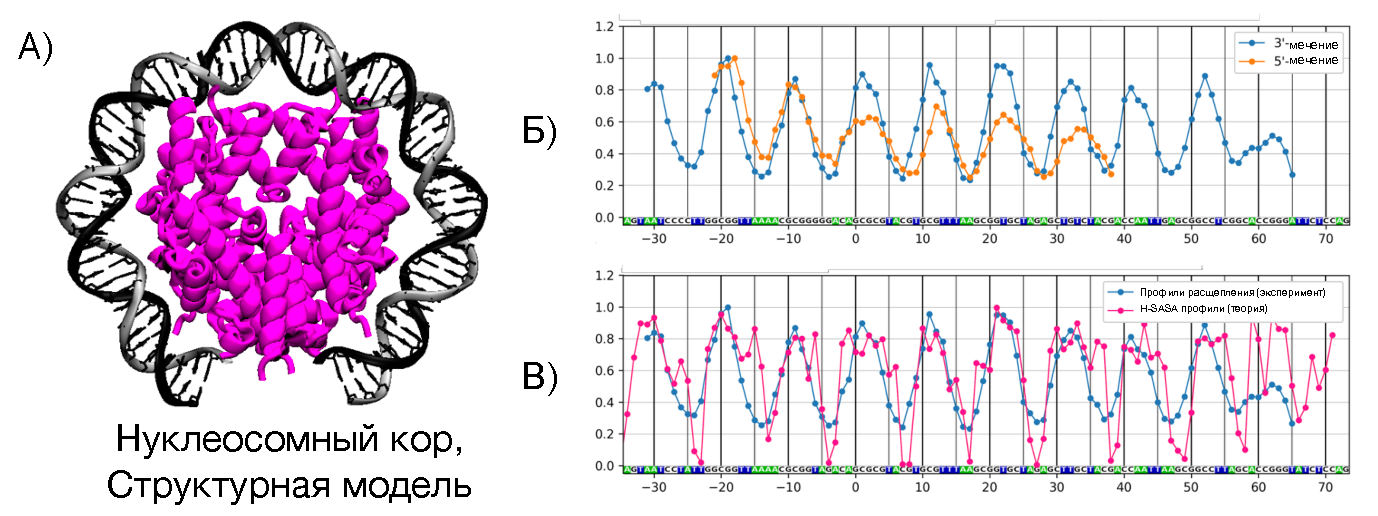
\includegraphics[width=\textwidth]{images/p5/part5_1_np/p5_1_f6.pdf}
    \caption[Экспериментальные и теоретические профили частоты расщепления ДНК гидроксильными радикалами в нуклеосомах]{\textbf{Экспериментальные и теоретические профили частоты расщепления ДНК гидроксильными радикалами в нуклеосомах.} A) Структура ДНК-белковых взаимодействий в нуклеосоме (из модели по гомологии нуклеосомы \textit{S. cerevisiae}, воссозданной на основе последовательности ДНК 601 на основе структуры PDB ID 3LZ0), показаны центральные 70 п.н. ДНК, гистоновые хвосты не показаны. ДНК демонстрирует периодический паттерн взаимодействий с октамером гистонов каждые 10-11 п.н. Б) Сравнение двух независимо полученных экспериментальных профилей для нуклеосом, восстановленных на последовательности ДНК 601/601TA, полученным в результате работы HYDROID. Профиль, ДНК меченной по 5'-концом, соответствует нуклеосомам, восстановленным на 601 позиционирующей последовательности с использованием гистонов из эритроцитов \textit{G. gallus} (эти данные доступны в HYDROID как Пример 2). 3'-меченный профиль соответствует нуклеосомам, воссозданным на аналогичной позиционирующей последовательности 601TA с использованием рекомбинантных гистонов центромерных нуклеосом \textit{S. cerevisiae} (эти данные доступны в HYDROID как Пример 1). Сравнение экспериментальных и H -SASA профилей для центромерной нуклеосомы \textit{S. cerevisiae}. Экспериментальный профиль такой же, как и профиль, у ДНК меченной по 5'-концу из панели B. Профиль H-SASA был получен с помощью HYDROIDpred с использованием модели  по гомологии центромерной нуклеосомы \textit{S. cerevisiae} на основе структруы PDB 3LZ0 (также доступной в примере 1).}
    \label{fig:p5_1_f6}
\end{figure}
    
    
    \subsection{Благодарности}

    Эта работа была поддержана программами внутренних исследований Национальной медицинской библиотеки и Национального института рака, Национальных институтов здоровья; Российским научным фондом [грант № 14-24-00031, договор № 14-24-00031-р] (разработка алгоритмов моделирования гелей и пакета HYDROID\_GUI); Медицинским институтом Говарда Хьюза Исследовательский кампус Джанелии и Университетом Джонса Хопкинса; Российско-американской программой сотрудничества в рамках программы приглашенных стипендиатов Национального института здоровья; грантами NIH  R01GM119398 и R21CA220151, R21DE025398 и P50DE019032. В этой работе использовались вычислительные ресурсы кластера NIH HPC Biowulf (http://hpc.nih.gov) и  вычислительные ресурсы центра высокопроизводительных вычислений МГУ им. М.В. Ломоносова.

    Мы благодарим Т. Туллиуса за ценные предложения, которые помогли сформулировать первоначальную идею этого исследования, Л. Заславского за обсуждения оптимальных алгоритмов аппроксимации данных и С. Миттернахта за изменения в программе FreeSASA.

    
% \begin{figure} [h!]
%     \centering
%     \includegraphics[width=\textwidth]{images/p5/part5_1_np/p5_1_f7.pdf}
%     \caption{}
%     \label{fig:p5_1_f7}
% \end{figure}
    
% \begin{figure} [h!]
%     \centering
%     \includegraphics[width=\textwidth]{images/p5/part5_1_np/p5_1_f8.pdf}
%     \caption{}
%     \label{fig:p5_1_f8}
% \end{figure}
    
    
    
    
    
    
    
    
    
    
    
    
    
    
    
    
    
    
    
    
    
    
    
    
    


\section{Создание моделей нуклеосом по данным гидроксильного футпринтинга}
\textit{Содержание данной главы следует статье \cite{shaytan_hydroxyl-radical_2017}}.


Нуклеосомы представляют собой наиболее распространенные комплексы белок-ДНК у эукариот, которые обеспечивают уплотнение геномной ДНК и участвуют в регуляции транскрипции, репликации и репарации ДНК. Детали позиционирования ДНК на нуклеосоме и конформации ДНК могут являться важными регуляторными сигналами. Метод футпринтинга комплексов белок-ДНК гидроксильными радикалами -- это химический метод, который позволяет исследовать организацию нуклеосом в растворе с высокой точностью, недостижимой другими методами. В этой работе мы предлагаем метод интегративного моделирования для построения атомистических моделей нуклеосом с высоким разрешением на основе экспериментов по гидроксильному футпринтингу. Наш метод точно определяет положение ДНК на нуклеосоме путем на основе данных футпринтинга для обеих цепей ДНК, используя свойства псевдосимметрии нуклеосомы. Мы провели эксперименты по гидроксильному футпринтингу с высоким разрешением для центромерных нуклеосом \textit{Saccharomyces cerevisiae}, структура которых является предметом дискуссий. Мы охрактеризовали эти структуры, используя наш подход интегративного моделирования. Наша модель обеспечивает основу для дальнейшего понимания взаимодействия между белком Cse4p и последовательносями аденинов (A-трактами), важными для функции центромеры в пекарских дрожжах.

\subsection{Введение}
Нуклеосомы - это элементарные строительные блоки хроматина, включающие сегмент ДНК, связанный с октамером гистоновых белков (H3, H4, H2A, H2B - по две копии каждого) \cite{kornberg_chromatin_1974-1}. Кор нуклеосомы (называемый, кором нуклеосомы или NCP) состоит из 145–147 п.н. ДНК, обернутых в виде $\sim$ 1,7 левых сверхспиральных витка вокруг октамера \cite{luger_crystal_1997} (рис. \ref{fig:p5:p5_2_f1}). Хотя общая структура нуклеосомы хорошо охарактеризована \cite{tan_nucleosome_2011}, каждая конкретная нуклеосома может значительно отличаться от своих аналогов за счет вариаций в последовательности ДНК, включения альтернативных вариантов гистонов \cite{draizen_histonedb_2016,shaytan_nucleosome_2015}, их посттрансляционных модификаций \cite{gardner_operating_2011} и взаимодействий с другими белками \cite{xiao_nonhistone_2011,becker_nucleosome_2013}. Эти изменения и вариации часто влияют на доступность и конформацию ДНК, которые, в свою очередь, модулируют основные процессы в хроматине, такие как транскрипция, репликация, репарация ДНК и т. д. \cite{gaykalova_structural_2015,luger_new_2012}. Смещение положения ДНК в нуклеосоме только на одну пару оснований приводит к изменениям в ее ротационном позиционировании примерно на 36 градусов, что может быть достаточно, чтобы повлиять на связывание многих белков с нуклеосомами, считывающими последовательность ДНК (например, пионерские факторы транскрипции \cite{iwafuchi-doi_pioneer_2014,cui_rotational_2014}). Следовательно, детальная структурная характеристика нуклеосом имеет большое значение. Атомные структуры отдельных нуклеосом получались с помощью рентгеновской кристаллографии \cite{tan_nucleosome_2011}. Однако этот метод требует очень много времени и во многих случаях сильно ограничен ограничениями по кристаллизации, составу и конформации нуклеосомы, потенциально приводя к конформациям, отличным от тех, которые могут быть в растворе. Поэтому очень востребованы точные и универсальные методы характеристики структур нуклеосом.
В лаборатории широко используются определенные биохимические методы для быстрой характеристики доступности и расположения ДНК на нуклеосомах в растворе. В этих методах используется визуализация ``следа'' белков на ДНК - разрезание ДНК ферментами или химическими веществами. Эти методы позволяют картировать взаимодействия белок-ДНК и охарактеризовать конформацию ДНК вдоль последовательности ДНК. Метод гидроксил-радикального футпринтинга (HRF) признан методом, обеспечивающим наивысшее разрешение благодаря небольшому размеру и нейтральной природе гидроксильных радикалов, приводящих к независимому от типу оснований расщеплению ДНК \cite{jain_footprinting_2008-1}. Считается, что разрыв цепи ДНК во время HRF происходит в основном за счет отщепления атомов водорода дезоксирибозы (рис.\ref{fig:p5:p5_2_f2}) \cite{pogozelski_oxidative_1998}. HRF обычно выполняется в несколько этапов: (а) каждая цепь ДНК метится на одном конце радиоактивным (или флуоресцентным) зондом; (б) комплекс белок-ДНК (или свободную ДНК) обрабатывают гидроксильными радикалами, которые расщепляют ДНК в открытых участках в режиме кинетики одиночного разрезания (по одному разрезу на цепь); (в) комплекс белок-ДНК можно снова очистить; (г) ДНК затем очищают от белков, денатурируют и подвергают денатурирующему электрофорезу в полиакриламидном геле высокого разрешения (ПААГЭ); (д) интенсивность каждой полосы (т. е. положения основания) на геле должна быть пропорциональна частоте расщепления ДНК во время реакции расщепления на конкретном нуклеотидном сайте \cite{jain_footprinting_2008-1}. Отображение каждой полосы в конкретное положение вдоль последовательности ДНК может быть легко выполнено путем электофореза продуктов реакций секвенирования ДНК (например, реакций Максама-Гилберта) на соседних дорожках.
Применение HRF к нуклеосомам было впервые предложено Hayes et al. задолго до появления первых рентгеновских структур нуклеосом с атомным разрешением \cite{hayes_structure_1990,hayes_histone_1991-1,hayes_histone_1991,churchill_detection_1990}. Эти авторы смогли оценить спиральную периодичность ДНК в нуклеосомах, и их работа с тех пор послужила эталоном для многих других исследований, в которых для характеристики нуклеосом использовался метод футпринтинга гидроксильными радикалами. В последних исследованиях использовались нуклеосомы с альтернативными последовательностями ДНК \cite{widlund_nucleosome_1999,bjorklund_attenuation_2006,morozov_using_2009}, связями между нитями ДНК, введенными химиотерапевтическими агентами \cite{bjorklund_attenuation_2006}, нуклеосомы, взаимодействующие с ремоделерами \cite{schwanbeck_spatial_2004} или другими белками \cite{syed_single-base_2010}. Хотя метод HRF в нуклеосомах, несомненно, помог охарактеризовать расположение нуклеосом, геометрию ДНК и сайты взаимодействия с нуклеосомосвязывающими белками, существует дополнительный потенциал этого метода, который можно задействовать.
Этот потенциал заключается в количественной оценке данных HRF и объединении этих данных с методами интегративного молекулярного моделирования для получения моделей нуклеосом на атомном уровне. Молекулярное моделирование нуклеосом является сложной задачей, поскольку оно требует не только моделирования октамера гистонов, но также включает в себя поиск правильного ротационного и трансляционного позиционирования ДНК по отношению к октамеру. Предыдущие исследования показали, что определенные нуклеосомы в дрожжах хорошо позиционированы, особенно центромерные \cite{cole_centromeric_2011}, и поэтому скольжение нуклеосомной ДНК только на одну пару оснований может привести к значительным изменениям в ее экспозиции. Частоты расщепления ДНК, извлеченные из экспериментов HRF в растворе, обычно имеют разрешение в один нуклеотид и могут предоставить данные об относительной доступности ДНК для расщепления, на которое влияют взаимодействия с белками и / или конформация ДНК (например, узкая малая бороздка). Экспериментальные данные HRF могут предоставить удобный источник данных для проверки и уточнения нуклеосомных моделей.
Основа для связи экспериментальных данных футпринтинга с молекулярным моделированием была сформулирована Balasubramanian et al. которые предположили, что частоты разрыва цепи ДНК гидроксильными радикалами были пропорциональны доступной для растворителя площади поверхности атомов водорода дезоксирибозы, рассчитанной по известным структурам \cite{balasubramanian_dna_1998}. Это облегчило интерпретацию профилей HRF с точки зрения количественных показателей, ширины больших и малых бороздок ДНК и других геометрических характеристик ДНК \cite{bishop_map_2011,pastor_detailed_2000}. Насколько нам известно, этот подход еще не применялся систематически к нуклеосомам. В качестве альтернативы Бегусова и соавт. предложили сложный гибридный подход к моделированию, основанный на моделировании методом Монте-Карло диффузии гидроксильных радикалов в сочетании с учетом параметров реакционной способности, полученными из подгонки моделей к экспериментальным данным \cite{begusova_radack_2001,begusova_radiolysis_2000}.
Ограниченный прогресс в использовании данных HRF для построения надежных моделей нуклеосом частично связан с отсутствием исследований, которые пытаются напрямую связать данные футпринтинга нуклеосом с рентгеновскими структурами высокого разрешения и динамикой нуклеосом. Другой причиной является недостаток методологий для количественной оценки экспериментальных профилей HRF нуклеосом и понимания потенциальных источников систематических ошибок и вариаций в экспериментальных данных.
В текущем исследовании мы пытаемся решить вышеупомянутые проблемы с целью предоставить надежный способ построения моделей нуклеосом на основе данных HRF и понять потенциальные различия между структурами нуклеосом, в кристаллических структурах и в растворах. Первая часть нашей работы посвящена теоретической оценке профилей HRF из трехмерных структур и их рационализации с точки зрения конформации ДНК и взаимодействий белок-ДНК. В частности, этот анализ позволил установить связь между псевдосимметрией нуклеосомы и сходством профилей HRF комплементарных нитей ДНК. Во второй части нашей работы мы выполнили HRF с высоким разрешением в растворе для двух разных систем на основе центромерных нуклеосом \textit{S. cerevisiae}, собранных \textit{in vitro} и содержащих вариант гистона Cse4 / CENP-A с различными последовательностями ДНК: центромерной последовательности ДНК из хромосомы III (CEN3) и хорошо позиционирующей последовательностью 601TA. Основываясь на экспериментальных данных и данных моделирования, мы предлагаем новый простой интегративный метод определения положения ДНК в нуклеосомах (как ротационных, так и трансляционных) с разрешением в одну пару оснований. В нашем методе используются экспериментальные данные HRF для обеих цепей ДНК и псевдосимметрия нуклеосом. Наконец, мы применили наш метод для определения позиционирования ДНК в нуклеосомах (позиционирование нуклеосом) и построили структурную модель центромерной нуклеосомы \textit{S. cerevisiae}, собранной \textit{in vitro}, ДНК которой необычайно богата А-трактами, которые, как известно, имеют решающее значение для функционирования центромер. Мы обсуждаем значение нашей структурной модели для функции центромеры.

\begin{figure}[H]
\centering
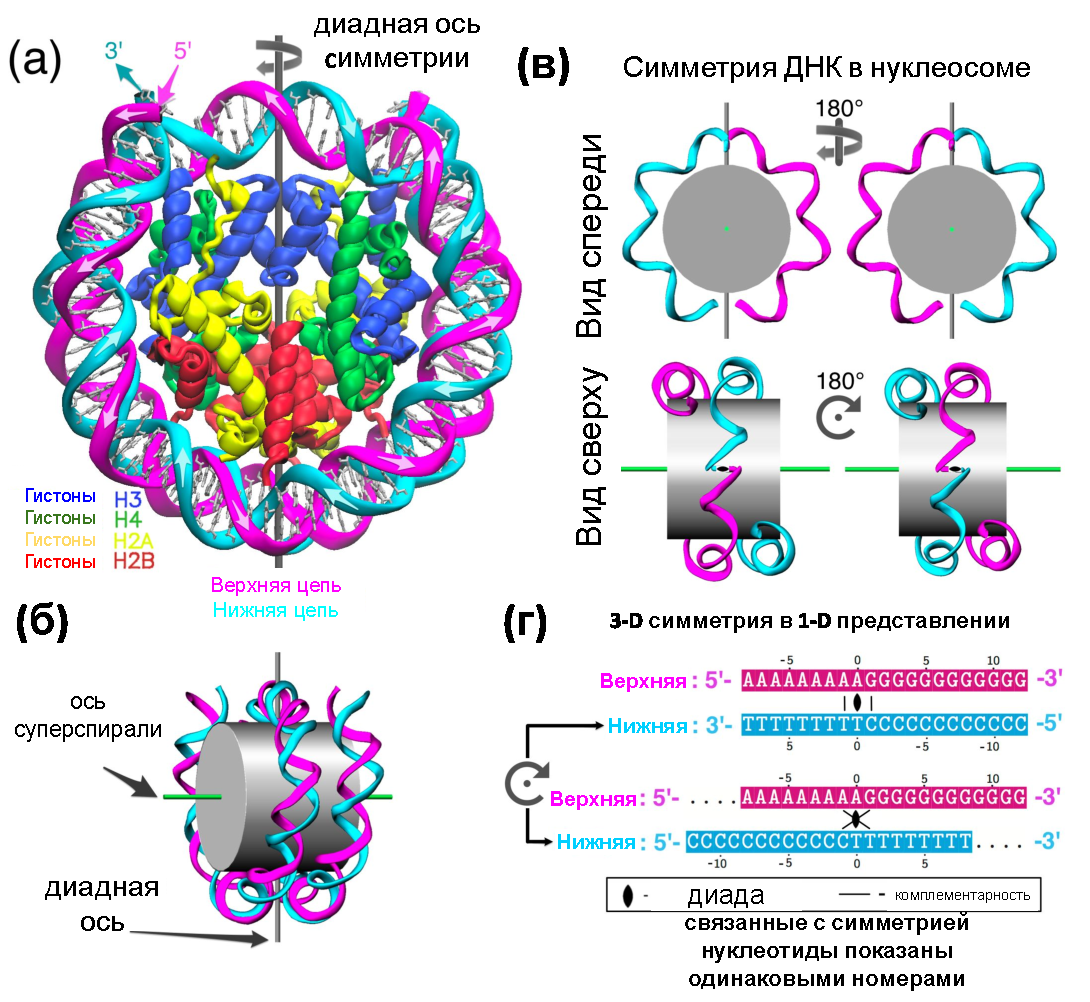
\includegraphics[width=\textwidth]{images/p5/part5_2_nar/p5_2_f1.pdf}
\caption[Структура нуклеосом и псевдосимметрия верхней и нижней цепей ДНК.]{
Структура нуклеосом и псевдосимметрия верхней и нижней цепей ДНК. (а) Представление структуры нуклеосомного кора (PDB 1KX5 (\cite{davey_solvent_2002})). (б) Схематическое изображение нуклеосомы, показывающее расположение оси псевдосимметрии второго порядка и сверхспиральной оси. (в) Иллюстрация псевдосимметричного отношения между верхней и нижней цепями ДНК в нуклеосоме (показаны только части цепей ДНК). (г) Изображение пространственной симметрии ДНК на плоских диаграммах последовательности: обычное представление (вверху) и сонаправленное (внизу). В последнем представлении две нити выровнены путем размещения диадных нуклеотидов верхней и нижней цепей ДНК одного под другим; следовательно, все связанные симметрией пары нуклеотидов верхней и нижней цепей ДНК также выровнены (один под другим). Комплементарность оснований между выбранными нуклеотидами показана на обоих изображениях.}
\label{fig:p5:p5_2_f1}
\end{figure}

\begin{figure}[H]
    \centering
    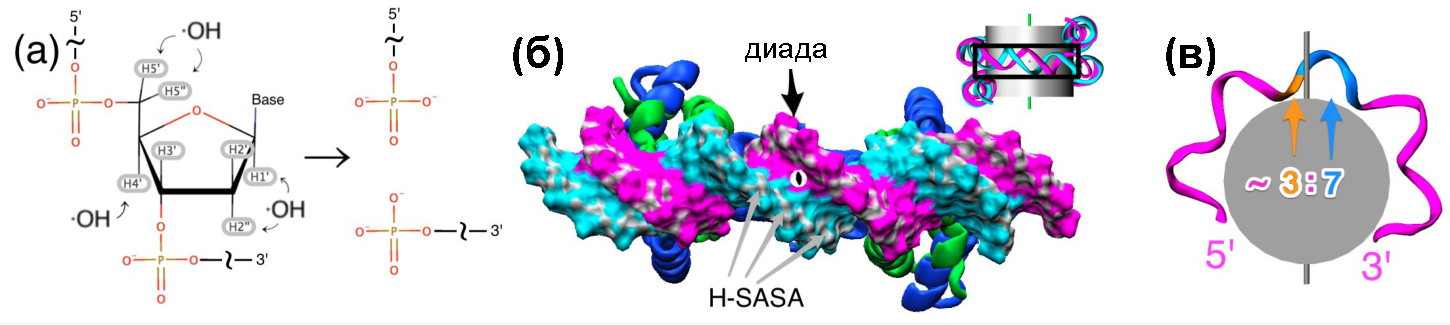
\includegraphics[width=\textwidth]{images/p5/part5_2_nar/p5_2_f2.pdf}
    \caption[Детали гидроксил-радикальных взаимодействий с нуклеосомной ДНК.]{Детали гидроксил-радикальных взаимодействий с нуклеосомной ДНК. (а) Химическая реакция гидроксильных радикалов с основной цепью ДНК: атомы водорода дезоксирибозы (выделены серым) атакуются, что приводит к разрушению остатка дезоксирибозы и расщеплению ДНК. Показаны только основные продукты расщепления. (б) Сегмент нуклеосомы, рассматриваемый сверху (см. Вставку) в представлении площади поверхности, доступной для растворителя (SASA). Участки SASA, принадлежащие атомам водорода дезоксирибозы (H-SASA), окрашены в серый цвет. (в) Асимметрия контактов гистон-ДНК относительно положения оси диады приводит к ее проявлению на профилях расщепления ДНК. Диада делит сегмент цепи ДНК между двумя соседними сайтами связывания на неравные части с соотношением $\sim$ 3:7 при подсчете в направлении 5$^\prime$-3$^\prime$. }
    \label{fig:p5:p5_2_f2}
\end{figure}

\subsection{Материалы и методы}
\subsubsection{Экспериментальные процедуры}

\emph{Приготовление фрагментов ДНК.} ДНК 601-TA была амплифицирована полимеразной цепной реакцией (ПЦР) с асимметричным сайтом рестрикции AvaI, CTCGGG, на обоих концах и клонирована в модифицированный вектор pUC19, который содержит сконструированный асимметричный сайт AvaI. Однако в исследовании ПЦР-амплификация высоко AT-богатой (~ 90\%) центромерной ДНК пекарских дрожжей была проблематичной. Таким образом, фрагмент ДНК CEN3 был химически синтезирован с асимметричным сайтом AvaI и клонирован в вектор pUC57 (Genscript USA Incorporated, Пискатауэй, Нью-Джерси, США). Асимметричный сайт AvaI использовали для лигирования фрагментов ДНК в тандемные массивы. Такие тандемные массивы фрагментов ДНК 601-ТА и центромеры затем клонировали в модифицированном векторе pUC19 с сконструированным асимметричным сайтом AvaI. Для крупномасштабного получения фрагментов ДНК плазмиды, которые содержат тандемные массивы, трансформировали в клетки DH5-$\alpha$ или XL1-Blue для стабильного размножения длинных тандемных массивов фрагментов ДНК. Очищенные плазмиды переваривали рестрикционным ферментом AvaI, и фрагменты очищали электрофорезом в агарозном геле и осаждали этанолом. Нуклеотидный состав четерехнуклеотидного выступа асимметричного сайта AvaI различается между верхней цепью (TS) и нижней цепью (BS), и, таким образом, может использоваться для мечения фрагментов ДНК, специфичных для цепи на 3$^\prime$-конце  с использованием радиоактивно или флуоресцентно меченных нуклеотидов в реакциях с использованием полимеразы Кленова. Поскольку ПЦР проблематична для получения AT-богатого фрагмента центромеры, 5$^\prime$-мечение любого конца потребовало бы химического повторного синтеза ДНК центромеры с дополнительными фланкирующими сайтами рестрикции и создания тандемных массивов для получения крупномасштабной ДНК; по этой причине маркировка 5$^\prime$ не проводилась.

\emph{Подготовка и восстановление нуклеосом}. Экспрессия и очистка коровых гистонов \textit{S. cerevisiae} проводились, как описано ранее \cite{xiao_nonhistone_2011,dyer_reconstitution_2004,mizuguchi_nonhistone_2007}. Октамеры гистонов были восстановлены с использованием известных протоколов \cite{dyer_reconstitution_2004}. Вкратце, эквимолярные количества очищенных рекомбинантных гистонов (H2A, H2B, Cse4 и H4) растворяли в денатурирующем буфере (7M гуанидин-HCl, 20 мМ трис-Cl, pH 7,5, 10 мМ дитиотреитол (ДДТ)) в концентрации 2 мг/мл. Смеси диализовали против четырех замен по 2 литра каждого буфера для рефолдинга (10 мМ Трис-Cl, pH 7,5, 1 мМ ЭДТА, 5 мМ бета-меркаптоэтанол, 0,1 мМ фенилметилсульфонилфторид (ФМСФ)), содержащий 2 М NaCl в течение 2 дней при $4^{\circ}$C. Затем смесь центрифугировали при 15 000 об / мин в микроцентрифуге Tomy MX-300 для удаления любого нерастворимого материала. Растворимые октамеры очищали фракционированием по размеру на колонке для гель-фильтрации Superdex 200. Фрагмент ДНК 601TA 157 п.н. \cite{cloutier_dna_2005} и фрагмент ДНК CEN3 136 п.н. получали, как описано ранее \cite{xiao_nonhistone_2011}. Их полноразмерные последовательности представлены на оси последовательностей на всех соответствующих рисунках. Для воссоздания нуклеосом очищенные октамеры гистонового кора и ДНК смешивали в 50 мкл высокосолевого буфера (2M NaCl, 10 мМ Tris-Cl, pH 7,5, 1 мМ EDTA, 0,02\% NP-40, 5 мМ бета-меркаптоэтанола) с добавлением бычьего сывороточного альбумина 400 мкг / мл. Смесь переносили в диализную установку SlideA-Lyzer MINI (Thermo Scientific). Блок для диализа помещали в контейнер с 600 мл высокосолевого буфера и диализовали в течение 30-60 минут с последующим диализом в солевом градиенте, в течение которого низкосолевой буфер (100 мМ NaCl, 10 мМ трис-Cl, pH 7,5, 1 мМ ЭДТА, 0,02\% NP-40, 2 мМ бета-меркаптоэтанол) закачивали в контейнер со скоростью 3,5 мл / мин в течение 16 часов. Затем диализный блок переносили в буфер с низким содержанием соли и диализовали в течение 60 мин. Диализ проводили при комнатной температуре, а образцы дополнительно обрабатывали при $65^{\circ}$C в течение ночи. 

\emph{Гидроксильный футпринтинг}. Нуклеосомы собирали на основе фрагментов ДНК, меченных по 3$^\prime$-концам с помощью $^{33}$P-dTTP для верхней цепи и $^{33}$P-dATP для нижней цепи, путем заполнения асимметричного сайта AvaI с использованием полимеразы Кленова. HRF нуклеосом выполняли на нуклеосомах с помощью реагента железо (II)-EDTA, как описано ранее \cite{schwanbeck_spatial_2004}. Продукты реакции разделяли на 1,3\% нативном агарозном геле, полосы, содержащие свободные нуклеосомы, визуализировали с помощью окрашивания SYBR Green и вырезали из геля. ДНК выделяли из срезов геля и разделяли на 8\% геле для секвенирования ДНК (National Diagnostics, каталожный номер EC-833). Маркерами подвижности ДНК были реакции секвенирования G + A и C + T тех же $^{33}$P-меченных фрагментов ДНК, которые выполнялись, как описано в Molecular Cloning, CSHL. Гели запускали на 40-сантиметровой стеклянной пластине при 1500-1600 В в течение ~70 минут при температуре геля около $55^{\circ}$C, затем переносили на фильтровальную бумагу DEAE (бумага для ионообменной хроматографии Whatman Grade DE81 от GE Life Sciences) и сушили под вакуумом. Радиоактивные сигналы регистрировались с помощью PhosphorImager (Fuji Photo Film Co., Ltd) и сканера Typhoon (Typhoon 9410, Amersham Biosciences).

\subsubsection{Вычислительный анализ}
\emph{Количественная оценка изображений гелей в экспериментах по футпринтингу гидроксильными радикалами}. Профили интенсивности 1D дорожек для каждой дорожки в геле были извлечены с помощью ImageJ v. 1.51f \cite{schneider_nih_2012}. Линия или ломанная линия была проведена вручную через центры всех полос в дорожке. Ширина линии была установлена примерно на половину ширины дорожки, а профиль сигнала вдоль полосы был извлечен и сохранен в отдельный файл для дальнейшей обработки. Эта стандартная процедура автоматически запускает выпрямление изображения для каждой полосы и усреднение данных по ширине полосы, как это реализовано в ImageJ. Профили интенсивности полос, соответствующие экспериментам с гидроксильными радикалами, были дополнительно проанализированы с помощью нашего недавно разработанного пакета HYDROID (доступного по адресу \url{https://github.com/ncbi/HYDROID}) (публикация в стадии подготовки), чтобы получить значения интенсивности расщепления ДНК. в каждой позиции в последовательности ДНК. Хотя наша методология основана на идеях, предложенных в более ранних работах \cite{shadle_quantitative_1997,takamoto_semi-automated_2004,das_safa_2005}, она имеет несколько новых аспектов. Во-первых, начальные местоположения пиков интенсивности, соответствующих полосам геля, были полуавтоматически назначены и сопоставлены с положениями вдоль последовательности ДНК путем сравнения их с полосами, полученными в результате реакций Максама-Гилберта \cite{jain_footprinting_2008-1}. Диапазон данных на каждом профиле HRF был установлен на область, в которой можно было идентифицировать непрерывный набор отдельных положений полос (либо непосредственно по наличию пика, либо иным образом однозначно выведенный из положения соседних пиков или соответствующих положений полос на других дорожках геля). Затем аналитическая функция была использована для аппроксимации экспериментального профиля HRF. Он представляет собой линейную комбинацию функций Гаусса, каждая из которых предназначена для описания формы определенной полосы на экспериментальном профиле. Алгоритм аппроксимации на основе метода наименьших квадратов Левенберга-Марквардта был использован для решения данной задачи. Параметры ширины функций Гаусса были ограничены, чтобы обеспечить монотонное уменьшение ширины с увеличением молекулярной массы расщепленных фрагментов ДНК, соответствующих полосам геля. Было показано, что такая регуляризация увеличивает точность процедуры аппроксимации и выполняется функцией, реализованной в HYDROID. Ранее функции Лоренца вместо функций Гаусса использовались в качестве эмпирического приближения для уменьшения искажений сигнала из-за авторадиографического метода детекции сигнала в геле (\cite{shadle_quantitative_1997} и приложение к нему). В нашем случае моделирование с помощью функций Лоренца дало несколько худшие результаты, измеренные по среднеквадратическому отклонению между аппроксимированными и экспериментальными кривыми, что оправдывает использование функций Гаусса для нашего анализа. В результате частоты расщепления ДНК для каждой позиции в последовательности ДНК были получены из значений коэффициентов (полученных интегрированием по интенсивностям для каждой полосы) перед функциями Гаусса, описывающими соответствующую полосу. Следует отметить, что профили интенсивности расщепления ДНК обычно различаются по абсолютной величине из-за их зависимости от многих экспериментальных условий (загрузка образца, время воздействия и т. д.). Чтобы обеспечить адекватное сравнение двух экспериментальных профилей, они должны быть в одном масштабе. С этой целью мы выполнили линейную регрессию, описав один профиль HRF как линейную функцию (без свободного члена) другого профиля. Значения последних значений профиля интенсивности затем были масштабированы с помощью полученного коэффициента линейной регрессии и нормализованы от нуля до единицы путем деления на максимальное значение интенсивности двух профилей. Для сравнения экспериментальных и теоретических (H-SASA, определение см. ниже) профилей использовалась простая нормализация каждого профиля по его максимальному значению.

\emph{Молекулярное моделирование и моделирование молекулярной динамики нуклеосом}. Моделирование молекулярной динамики (МД) различных нуклеосом было выполнено в соответствии с нашим протоколом, описанным в работе \cite{shaytan_coupling_2016} если не указано иное. Первоначальные модели были основаны на рентгеновских структурах, полученных из банка данных PDB, или на моделя созданных по гомологии. Первоначально структуры были ориентированы в системе координат нуклеосомы, как определено ранее \cite{shaytan_coupling_2016}, так что ось Z соответствовала суперспиральной оси ДНК (рис. \ref{fig:p5:p5_2_f1}Б). Моделирование проводилось в течение 80 нс, и моментальные снимки сохранялись каждые 1 нс, первые 30 нс МД моделирования отбрасывались как период релаксации. Атомы оснований N1 и N9 в ДНК были привязаны к их исходным положениям с помощью гармонических ограничений с константой жесткости в 6 ккал / моль / A$^2$. Кроме того, мы сравнили МД-траектории с микросекундной траекторией нуклеосомы с полными гистоновыми хвостами и без ограничений на ДНК опубликованой ранее \cite{shaytan_trajectories_2016}. Структуры были визуализированы и проанализированы с использованием VMD \cite{humphrey_vmd_1996}. Первоначальная структура центромерной нуклеосомы \textit{S. cerevisiae} содержащей белок Cse4p с последовательностью ДНК 601TA (601TA-NUC) была построена на основе структуры нуклеосомы \textit{X. laevis} с 601-ой ДНК (PDB ID: 3LZ0) с использованием Modeller \cite{sali_comparative_1993} и 3DNA. Последовательности гистонов были получены из базы данных HistoneDB 2.0 \cite{draizen_histonedb_2016}. Модель центромерной нуклеосомы дрожжей на последовательности ДНК CEN3 (CEN3-NUC) была построена с использованием тех же методов на основе структуры нуклеосомы \textit{X. laevis} с $\alpha$-сателлитной  ДНК (PDB ID: 1KX5). Поскольку нет данных о позиционировании ДНК для этой нуклеосомы, мы определили его, используя наш метод определения диады, примененный к экспериментальным данным HRF для CEN3-NUC (см. ниже). В обеих моделях ДНК моделировали с использованием центрального фрагмента длиной 120 п.н. (60 п.н. от диады в каждом направлении) - фрагмента, который, как известно, однозначно организован центромерными нуклеосомами \cite{tachiwana_crystal_2011}. 

\emph{Теоретическая оценка частотных профилей расщепления ДНК по атомным структурам}. Как предложено в  \cite{balasubramanian_dna_1998}, профили частоты расщепления нуклеосомной ДНК были теоретически оценены как сумма площадей, доступных для растворителя (SASA) для всех атомов водорода дезоксирибозы данного нуклеотида, в дальнейшем называемые профилями H-SASA. Расчеты SASA были выполнены с использованием программы NACCESS \cite{hubbard_naccess_1993} с радиусом зонда 1,4 A, шириной среза 0,005 A и радиусами атомов, установленными в параметрах rmin силового поля CHARMM36 \cite{best_optimization_2012}. Для систем с усеченными гистоновыми хвостами хвосты были усечены в следующих N-концевых (H3G44, H4D24, H2A16T и H2BR33) и C-концевых (H2AK118) положениях (нумерация остатков дана в системе отсчета канонических гистонов \textit{X. laevis}. По умолчанию профили H-SASA были усреднены по 50 снимкам МД (с интервалом каждые 1 нс) полностью гидратированных структур (по причинам, описанным в разделе ``результаты''). Для моделирования МД атомы водорода добавлялись в ходе подготовки системы к моделированию, а в случаях прямого анализа рентгеновских структур положения атомов водорода генерировались с помощью REDUCEv.3.14 из AmberTools13 \cite{word_asparagine_1999}. Графики профилей вместе с последовательностями были созданы с помощью ggplot \cite{wickham_ggplot2_2009} и TexShade \cite{beitz_texshade_2000}. Усечение гистоновых хвостов и релаксация структуры и усреднение, обеспечиваемые моделированием МД, сыграли важную роль в получении профилей H-SASA, которые отражали периодичность ДНК в нуклеосомах (см. Раздел ``Результаты''). Вклад контактов ДНК-белок в профили H-SASA оценивали путем расчета профилей H-SASA для нуклеосомной ДНК с удаленными гистонами. Можно видеть, что модель H-SASA чувствительна к сужению малой бороздки ДНК в определенных местах ДНК-гистоновых взаимодействий, где ДНК изгибается в сторону малой бороздки. Однако контакты гистон-ДНК вносят основной вклад в минимумы H-SASA на этих сайтах.

\emph{Расчет параметров геометрии ДНК}. Параметры, которые представляют пространственную ориентацию, конформацию и периодичность нуклеосомной ДНК в виде одномерных профилей, являются важными инструментами нашего анализа. В качестве основного параметра, отражающего ориентацию пар оснований ДНК в нуклеосомной суперспирали, мы использовали величину относительного кручения нуклеосомной ДНК (relative twist, rTw). Два типа параметров кручения для характеристики суперспиральной ДНК в нуклеосоме были определены ранее: внутреннее кручение (iTw) и rTw (или локальное кручение) \cite{richmond_structure_2003,travers_dna_1993}. Предполагается, что последний измеряется в экспериментах по HRF или ферментативному расщеплению, потому что он подчеркивает геометрически эквивалентные положения вдоль суперспирали ДНК. iTw, с другой стороны, выделяет только собственное вращение пар оснований относительно друг друга вдоль ДНК. Однако известно, что значения rTw и iTw связаны через сверхспиральный шаг нуклеосомной ДНК \cite{travers_dna_1993}. Значения iTw для каждого шага пары оснований были рассчитаны с использованием 3DNA \cite{lu_3dna_2008}; суммирование этого значения по последовательности ДНК дало совокупное значение iTw (ciTw). Чтобы охарактеризовать rTw, мы вводим здесь новую величину - угол ориентации пары оснований (BPOA), предназначенный для отражения локальной ориентации нуклеотидов относительно октамера гистонов. BPOA был рассчитан из атомистических структур нуклеосом следующим образом: (i) суперспиральная ось нуклеосомы (рис. \ref{fig:p5:p5_2_f1}Б) была определена, как описано в работе \cite{shaytan_coupling_2016}; (ii) для каждого нуклеотида был определен вектор пары оснований (BPV) как вектор, указывающий от гликозидного атома азота текущего нуклеотида к соответствующему атому комплементарного нуклеотида (таким образом соединяя атомы N1 и N9); (iii) для каждого нуклеотида его соответствующий центр пары оснований (BPC) определяли как среднюю точку BPV; (iv) BPOA затем определяли как угол между BPV и перпендикуляром, направленным от суперспиральной оси нуклеосомы к BPC (радиальный вектор в цилиндрической системе координат). Значения BPOA служили мерой rTw в диапазоне от 0 до 180$^\circ$. По аналогии с ciTw, кумулятивная rTw (crTw) была реализована путем суммирования вращения BPV вдоль последовательности и добавления 180$^\circ$ каждый раз, когда значение BPOA начинало новый интервал. Относительную (локальную) периодичность нуклеосомной ДНК в каждом конкретном положении рассчитывали на основе разницы значений crTw между сайтами на 5 п.н. выше и ниже выбранного положения. Альтернативный способ расчета rTw с использованием BPOA, определяемого как угол между BPV и плоскостью, перпендикулярной супспиральной оси, дал почти идентичные результаты, что подтвердило наш выбор BPOA в качестве меры rTw. Разница между crTw и ciTw наблюдалась в соответствии с теоретическими ожиданиями. Мы использовали параметр rTw для характеристики пути ДНК в атомистических структурах NCP и для расчета локальной периодичности вдоль последовательности ДНК. Это позволило нам подробно проанализировать вращательное позиционирование ДНК в нуклеосомах и идентифицировать геометрически эквивалентные положения относительно поверхности октамера. Минимумы кривой rTw соответствуют положениям, в которых соответствующие пары оснований ориентированы почти перпендикулярно сверхспиральной оси, а нуклеотид верхней цепи ДНК взаимодействует с октамером главным образом через его атомы основной цепи. Локальная периодичность ДНК для анализируемых структур (рисунки \ref{fig:p5:p5_2_f3}A и \ref{fig:p5:p5_2_f4}) колеблется между 10 и 11 п.н. на оборот, а ДНК чрезмерно скручена вокруг положений $\pm$20 и $\pm$50 (SHL $\pm$2 и $\pm$5), что находится в согласии с результатами статьи \cite{tan_nucleosome_2011}.


\subsection{Результаты}
\subsubsection{Анализ теоретических частотных профилей расщепления ДНК для разных нуклеосом}
Расчет теоретических профилей частоты расщепления HRF основан на предположении, что он определяется профилями HSASA (см. Раздел ``Материалы и методы'') \cite{jain_footprinting_2008-1}. Это, конечно, только приближение к сложным процессам диффузии и взаимодействия, происходящим во время реакции гидроксильного футпринтинга. Однако есть определенные соображения в пользу такого подхода. Это позволяет надежно оценить теоретические профили с разрешением до одиночных нуклеотидов на основе атомных нуклеосомных структур или точных структурных моделей и сделать важные выводы об ожидаемой форме и сходстве экспериментальных профилей. Мы утверждаем, что симметрия нуклеосом может быть использована, чтобы обеспечить способ проверки и повышения точности теоретических профилей, облегчить интерпретацию экспериментальных профилей HRF и позволить идентифицировать диаду нуклеосом из экспериментальных данных HRF. Действительно, нуклеосомы обладают осью псевдосимметрии второго порядка (рис. \ref{fig:p5:p5_2_f1}Б-Г), которая связывает верхнюю и нижнюю цепи нуклеосомной ДНК таким образом, что если нуклеосома повернута на $180^{\circ}$ вокруг оси диады, то верхняя цепь ДНК почти точно совпадет с положением нижней цепи и наоборот. В частности, 5$\prime$-конец верхней цепи будет совмещен с 5$\prime$-концом нижней цепи. Сначала мы исследовали структуру с самым высоким разрешением (PDB ID: 1KX5 \cite{davey_solvent_2002}), где симметрия октамера гистонов дополняется симметрией квазипалиндромной последовательности ДНК: центральная пара оснований на диаде подразделяет нуклеосому и двухцепочечную ДНК на две идентичные половины. В случае известных структур точное положение диады можно непосредственно рассматривать как единственную пару оснований, расположенную на оси псевдосимметрии \cite{luger_crystal_1997}. На рис. \ref{fig:p5:p5_2_f3} показана четкая картина периодичности профилей H-SASA, рассчитанных на основе этой структуры для обеих цепей ДНК. Эта форма и периодичность очень похожи для обеих цепей ДНК, учитывая симметрию системы. Ось диады делит сегмент между двумя минимумами на графике H-SASA на неравные части (примерно в соотношении 3:7) с расположением диады ближе к 5$^\prime$ концу цепи ДНК. Это является следствием геометрии нуклеосомы и проиллюстрировано на рисунках \ref{fig:p5:p5_2_f2}Б и В. На рисунке \ref{fig:p5:p5_2_f3}В профиль H-SASA имеет отчетливые резкие минимумы в каждой позиции, где ДНК ориентирована перпендикулярно поверхности октамера, и довольно похожие на плато области высоких значений подверженности потенциальной атаке гидроксильных радикалов между этими позициями. Расстояние между минимумами на профиле H-SASA соответствует периодичности 10–11 п.н., но положения минимумов H-SASA не всегда точно соответствуют положениям минимумов rTw - они обычно отклоняются на 1 или 2 позиции в любом направлении. Последнее подчеркивает тот факт, что не только кручение ДНК отвечает за точную форму профилей H-SASA, но и различия во взаимодействиях белок-ДНК в различных сайтах связывания ДНК на нуклеосомах влияют на локальные положения минимумов H-SASA. Чтобы получить представление об этих вариациях, мы рассчитали индивидуальный вклад аминокислот в защиту ДНК от гидроксильных радикалов, рассчитанный как изменение общего H-SASA после удаления одного определенного аминокислотного остатка. Хорошим примером локального изменения формы H-SASA является повышенная защита в профилях в положении -43, проявляющаяся в виде локального минимума на рисунке \ref{fig:p5:p5_2_f3}В, который вызван взаимодействиями ДНК с $\alpha$N-спиралью, уникальной для H2A. Несмотря на наличие локальных выбросов, общие профили H-SASA двух цепей ДНК демонстрируют хорошую суперпозицию. Как упоминалось ранее, это результат почти идеальной симметрии данной нуклеосомы как на уровне белка, так и на уровне ДНК. Эксперименты HRF проводятся в растворе на ансамбле нуклеосом, которые в совокупности представляют конформационное пространство, доступное отдельным нуклеосомам в течение длительных периодов времени, поэтому уместно предположить, что две идентичные копии гистонов и хвостов гистонов будут исследовать неразличимые ансамбли конформаций. Следовательно, введенное выше правило симметрии должно также соблюдаться. Гибкие гистоновые хвосты, которые часто встречаются в адсорбированных конформациях в структурах рентгеновских нуклеосом (если они разрешены) могут вносить асимметрию в профиль H-SASA и могут обеспечить значительную дополнительную защиту ДНК от расщепления. Мы обнаружили, что наилучшее совпадение профилей H-SASA, соответствующих двум нитям ДНК были получены, когда гибкие гистоновые хвосты были опущены и ансамблевое усреднение и релаксация остова ДНК была выполнена в ходе МД моделирования (Рисунок \ref{fig:p5:p5_2_f3}В). По этой причине мы реализовали протокол с использованием систем с усеченными гистоновыми хвостами и усреднение по ансамблю МД, который мы использовали на протяжении всего исследования. Далее мы проанализировали влияние вариаций последовательности ДНК на геометрию ДНК и теоретические H-SASA профили. Рисунок \ref{fig:p5:p5_2_f4} суммирует различия в геометрии ДНК и периодичности для трей доступных рентгеновских структуры нуклеосомного кора с разной ДНК последовательностью: $\alpha$-сателлитная ДНК длиной 146 п.н.  (``NCP146'') \cite{luger_crystal_1997}, модифицированная $\alpha$-сателлитная ДНК длиной 147 п.н. (``NCP147'') \cite{davey_solvent_2002}  и 601 высокоаффинная последовательность Видома длиной 145 п.н. (``NCP145'') \cite{lowary_new_1998,vasudevan_crystal_2010}. Во всех этих структурах одна пара нуклеотидов расположена строго на диаде и ДНК проходит один и тот же сверхспиральный путь, несмотря на различия в их длине. Это достигается за счет растяжения/сжатия ДНК на участках, расположенных на расстоянии $\pm$20 или $\pm$50 п.н. от диады. Это иллюстрируется относительной периодичностью параметра rTw, предложенного в этом исследовании (рис. \ref{fig:p5:p5_2_f4}, верхний график). В то время как молекулы ДНК из NCP147 и NCP145 принимают очень похожие конформации с обеих сторон нуклеосомы, ДНК из NCP146 растянута на 1 п.н. с одной стороны. Практически идентичная конформация ДНК по обе стороны диады в NCP147 и NCP145 приводит к очень хорошему наложению между профилями H-SASA для обеих нитей ДНК (коэффициент корреляции Пирсона = 0,97, Рисунок \ref{fig:p5:p5_2_f3}). Что касается NCP146, несмотря на небольшую асимметрию двух половин нуклеосомной ДНК, сходство профиля H-SASA между двумя цепями поддерживается в пределах $\pm$20 п.н. вблизи диады. Однако небольшая асимметрия NCP146 не будет проявляться на профилях HRF для ансамбля нуклеосом в растворе. На самом деле, NCP146, имеющая чисто палиндромную последовательность ДНК, не будет иметь предпочтений относительно того, с какой стороны нуклеосомной ДНК растягиваться или расширяться, потому что две половинки ДНК полностью идентичны.

\begin{figure}[H]
    \centering
    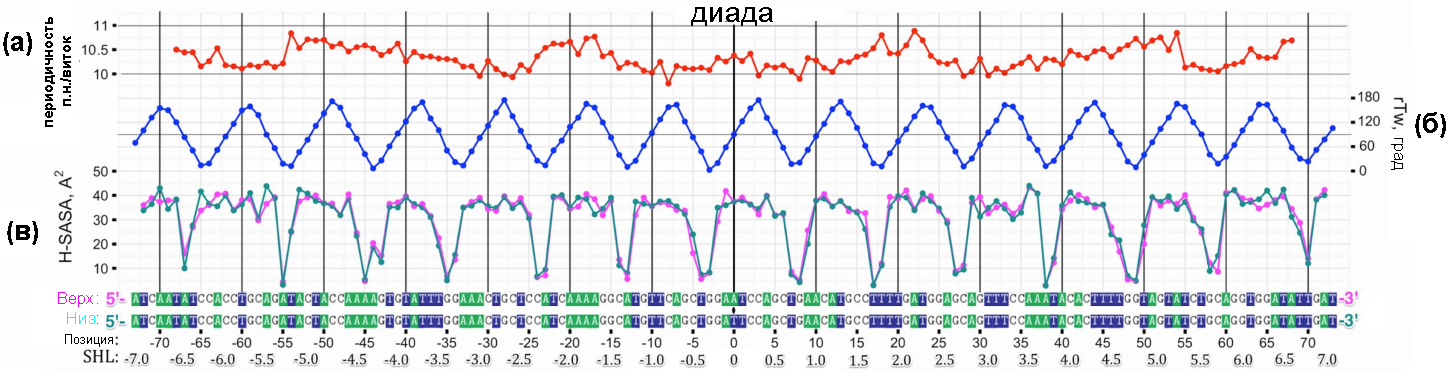
\includegraphics[width=\textwidth]{images/p5/part5_2_nar/p5_2_f3.pdf}
    \caption[Структура ДНК и профили H-SASA в рентгеновской структуре самого высокого разрешения NCP (NCP147)]{Структура ДНК и профили H-SASA в рентгеновской структуре самого высокого разрешения NCP (NCP147). (А) Локальная периодичность вращения ДНК в нуклеосоме, рассчитанная по относительному повороту (rTw). (Б) rTw нуклеосомной ДНК вдоль последовательности, нанесенный в направлении 5'-3' верхней цепи (TS). (В) Профили H-SASA для верхней цепи (пурпурный) и нижней цепи (голубой), оба профиля и последовательности под ними даны в направлении 5'-3'. Профили H-SASA рассчитаны по МД траектории NCP147 без гистоновых хвостов (см. Раздел ``Материалы и методы'').}
    \label{fig:p5:p5_2_f3}
\end{figure}

\begin{figure}[H]
    \centering
    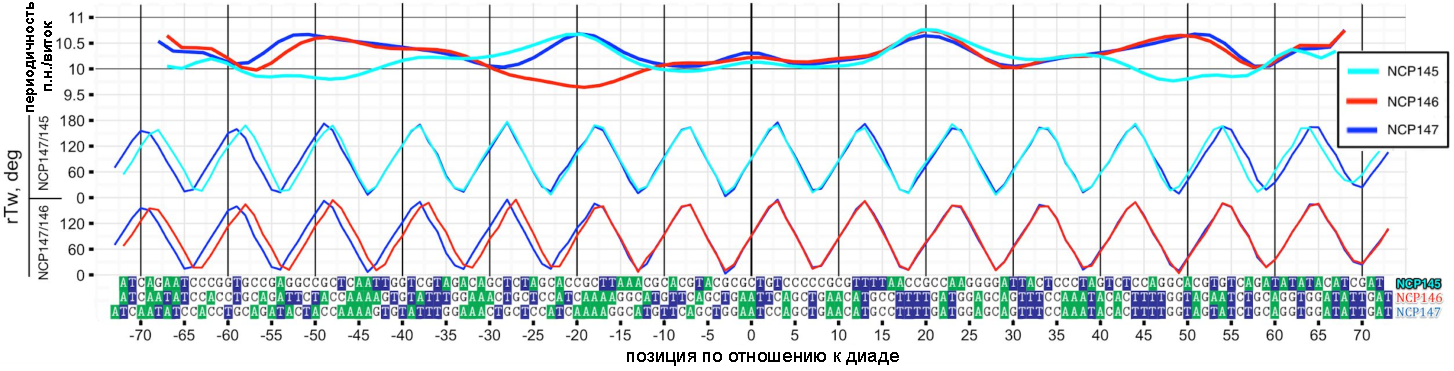
\includegraphics[width=\textwidth]{images/p5/part5_2_nar/p5_2_f4.pdf}
    \caption[Различия в структуре ДНК между разными рентгеновскими структурами нуклеосомы.]{Различия в структуре ДНК между разными рентгеновскими структурами нуклеосомы. Вверху: то же, что на рис. \ref{fig:p5:p5_2_f3}A, но сглаженный B-сплайном (с 30 степенями свободы). Внизу: попарное сравнение профилей rTw.}
    \label{fig:p5:p5_2_f4}
\end{figure}

\subsubsection{Количественная оценка экспериментальных профилей HRF и их сравнение с теоретическими профилями H-SASA}

Мы провели ряд экспериментов по гидроксильному футпринтингу для собранных \textit{in vitro} октамерных нуклеосом  на основе центромерных гистонов \textit{S. cerevisiae} и двух различных последовательностей ДНК: высокоаффинной последовательности 601TA и центромерной ДНК последовательность третьей хромосомы пекарских дрожжей CEN3 (601TA-NUC и CEN3-NUC). Кроме того, мы проанализировали свободную CEN3 ДНК (CEN3-free). Согласно нашей вычислительной процедуре, каждому положению в последовательности ДНК может быть присвоено значение относительной частоты расщепления гидроксильными радикалами путем количественной оценки экспериментально полученного изображения геля ПААГЭ для продуктов реакции HRF (Рисунок \ref{fig:p5:p5_2_f5}). В качестве доказательства концепции на рисунке \ref{fig:p5:p5_2_f5}В изображен экспериментальный профиль HRF 601TA-NUC  по сравнению с теоретическим профилем H-SASA, полученным из модели высокого качества с известной позицией диады созданной на основе рентгеноструктурных исследований (раздел ``Материалы и методы''). Общая периодичность экспериментальных и теоретические профилей хорошо согласуются между собой. Заметное уменьшение амплитуды сигнала к 3$\prime$ концу ДНК, вероятно, связано с пониженной склонностью коротких фрагментов ДНК к осаждению на стадии очистки. Экспериментальные профили для верхней и нижней цепи ДНК при наложении в 5$\prime$–3$\prime$ направлениях (рис. \ref{fig:p5:p5_2_f5}Г) очень похожи по форме, отражая псевдосимметрию нуклеосомы, как показано в предыдущем разделе.

Расположение минимумов в сайтах ДНК-гистоновых взаимодействий на H-SASA и экспериментальных профилях совпадают с точностью до $\pm$1 п.н., в большинстве случаев экспериментальные минимумы смещены к 5$^\prime$-концу цепи по отношению к минимумам H-SASA. Возможное объяснение состоит в том, что во время расщепления гидроксильным радикалом 3$^\prime$- меченой цепи ДНК в дополнение к основному продукту с 5$\prime$-фосфатным концом, как известно, присутствует второстепенный альтернативный продукт - цепь, оканчивающаяся 5$\prime$-альдегидной группой \cite{balasubramanian_dna_1998}. 5$^\prime$-альдегидный продукт, который образуется в результате отрыва 5$\prime$-атома водорода, на 1 нуклеотид длиннее, чем цепь с концевым 5$^\prime$-фосфатным концом, упомянутая выше, и она не имеет отрицательного заряда фосфатной группы и, таким образом, имеет подвижность в геле на 2–3 полосы медленнее по сравнению с соответствующим продуктами реакций Максама – Гилберта \cite{kappen_deoxyribonucleic_1983}. Таким образом, в фактически измеренном профиле частоты расщепления ДНК ожидается, что некоторая часть сигнала будет сдвинута на 2–3 пика в сторону 5$^\prime$-конца. Это может привести к небольшому смещению минимумов на измеренном профиле относительно истинного профиля (аппроксимированного профилем H-SASA). Упомянутый эффект должен быть значительно снижен, если нить ДНК радиоактивно помечена на 5$^\prime$-конце \cite{balasubramanian_dna_1998}, но создание 5-меченых фрагментов центромерной ДНК с высоким содержанием AT является технически сложной задачей (раздел ``Материалы и методы'').

Есть и другие важные различия между теоретически оцененными профилями H-SASA и экспериментальными. Последние демонстрируют гораздо более плавное изменение значений частоты расщепления вдоль последовательности, в то время как профили H-SASA имеют резкие минимумы шириной 1-2 п.н., окруженные областями с высокими значениями частоты расщепления (Рисунок \ref{fig:p5:p5_2_f5}В). Кроме того, хотя в определенных положениях значения H-SASA близки к нулю, что указывает на высокую защиту ДНК от расщепления, экспериментальные данные подтверждают минимальную частоту расщепления по меньшей мере в размере 25\% относительно максимальных значений. В дополнение к этому, экспериментальные профили HRF имеют отчетливые локальные максимумы, которые соответствуют ДНК, обращенной от октамера, в то время как профили H-SASA имеют форму плато в соответствующих областях. Возможные причины этих расхождений указаны в разделе ``Обсуждение'' ниже.

Мы наблюдали, что общий синусоидальный профиль футпринтинга ДНК в нуклеосомах имеет выбросы в определенных положениях пар оснований, их величина варьируется от эксперимента к эксперименту. Эти выбросы лучше всего проиллюстрированы на наборах данных нуклеосом CEN3-NUC и выделены стрелками на рисунке \ref{fig:p5:p5_2_f6}. Интересно, что расположение этих выбросов очень хорошо соответствует положениям выбросов на свободной ДНК. HRF свободной ДНК определяется в основном ее геометрией, которая зависит от последовательности. Необычная природа последовательности CEN3, которая очень богата A-трактами (определяемыми как четыре или более последовательных пары оснований A-T без шага TpA \cite{stefl_dna_2004}), проявляется в виде пиков в местах, где эти A-тракты нарушены гуанинами или цитозинами. Расположение основных пиков, наблюдаемых экспериментально для свободной ДНК CEN3, подтверждается прогнозами веб-сервера ORCHID, который предсказывает профили HRF путем усреднения существующих измерений HRF для всех возможных свободных тринуклеотидов \cite{greenbaum_construction_2007}. Тем не менее, не следует ожидать идеального соответствия между этими двумя методами, поскольку A-тракты характеризуются нелокальными разветвленными водородными связями, которые могут приводить к неаддитивным дальнодействующим, а не локальным эффектам, проявляемым в тринуклеотидах \cite{haran_unique_2009}. Появление аналогичных выбросов на HRF профилях нуклеосомальной ДНК, вероятно, связано с взаимодействием между внутренней геометрией и динамикой свободной ДНК и геометрией, наложенной на ДНК путем связывания с гистонами. Наше моделирование теоретических профилей расщепления с использованием МД-моделирования предполагает, что значения H-SASA довольно чувствительны к небольшим колебаниям двугранных углов основной цепи ДНК, которые могут быть вызваны только небольшими смещениями положений пары оснований. Это дает один потенциальный ключ к пониманию того, как небольшие изменения в структуре и динамике нуклеосом из-за вариации последовательности ДНК могут проявляться в профилях HRF.


\subsubsection{Новый метод определения положения нуклеосомной ДНК на основе данных гидроксильного футпринтинга}
Анализ как экспериментальных профилей, так и профилей H-SASA, описанных в предыдущих разделах, выявил несколько ключевых взаимосвязей между формой профилей HRF и положением ДНК на нуклеосоме. Описанный ниже метод идентификации диады основан на этих наблюдениях. Ось псевдосимметрии воторого порядка нуклеосомы (рисунок \ref{fig:p5:p5_2_f1}) связывает верхнюю и нижнюю цепи нуклеосомной ДНК так, что если нуклеосома повернута на 180$\circ$ вокруг диадной оси, то верхняя цепь ДНК накладывается на симметричное положение нижней цепи и наоборот (Рисунок \ref{fig:p5:p5_2_f1}В). Это наблюдение подразумевает, что профили HRF для верхней и нижней цепей ДНК должны совпадать (или быть очень похожими в зависимости от степень псевдосимметрии, как обсуждалось ранее), если оба профиля сравнивать в том же направлении (в нашем случае от 5$^\prime$ к 3$^\prime$). На основе H-SASA и экспериментальных профилей HRF, а также анализе геометрии структуры нуклеосомы, можно увидеть, что положение диады расположено асимметрично между двумя локальными минимумами на соответствующем профили любой из нитей ДНК. Диада делит отрезок между минимумами примерно в соотношении 3:7 (далее именуемое ``правилом соотношения 3:7'') (Рисунок \ref{fig:p5:p5_2_f1}В).
Важным аспектом является выбор правильных систем отсчета для сравнения профилей верхней и нижней цепей. Это особенно актуально, поскольку в профилях HRF обычно отсутствуют данные около концов нуклеосомной ДНК из-за ограниченного разрешения ПААГЭ, что делает невозможным идентифицировать нуклеосомную границу на каждом профиле и использовать ее в качестве маркера для их выравнивания. Однако, если известно положение диады в ДНК, также известны положения соответствующих нуклеотидов диады на каждом профиле. В этом случае, из-за геометрических причин и соображений комплементарности оснований цепи, правильный выбор систем отсчета может быть достигнут путем размещения положений нуклеотидов диады каждого профиля в 0, как показано на рисунке \ref{fig:p5:p5_2_f1}Г. Это проиллюстрировано на примере системы 601TA-NUC (рис. \ref{fig:p5:p5_2_f5}Г), где известное положение диады из структуры (см. Раздел ``Материалы и методы'') используется для построения экспериментальных профилей HRF для верхней и нижней цепей ДНК одной и той же системы в их соответствующих системах отсчета. Два профиля выглядят идеально выровненными (коэффициент корреляции Пирсона = 0,94), что подтверждает правильный выбор положения диады.
Если теперь представить себе ситуацию, когда положение диады неизвестно, но есть эксперименты по гидроксильному футпринтингу для обеих цепей ДНК, описанный выше подход можно легко обобщить для определения положения диады и, следовательно, общего позиционирования ДНК (также называемого позиционированием нуклеосом). Поскольку каждое значение интенсивности профиля HRF соответствует определенному основанию на цепи ДНК, выравнивание профиля определяет выравнивание последовательностей двух цепей, нанесенных на график в направлении от 5$^\prime$ к 3$^\prime$. Соответствующее положение диады на выравнивании последовательностей между верхней и нижней цепями ДНК затем может быть идентифицировано как единственное положение, где выровненные основания образуют пару оснований в структуре двухцепочечной нуклеосомной ДНК.
На практике производится выборка различных совмещений профилей HRF для верхней и нижней цепей ДНК, и качество их соответствия оценивается путем вычисления коэффициента корреляции между двумя выровненными профилями HRF (только перекрывающиеся части профилей используются для расчета коэффициента). Такой подход вдохновлен теорией обработки сигналов, в которой сходство между двумя процессами оценивается путем вычисления функции взаимной корреляции. Положение диады должно соответствовать максимуму (хотя бы локальному максимуму) коэффициента корреляции. Корреляция между двумя профилями HRF как функция предполагаемого положения диады для данных 601TA-NUC показана на рисунке \ref{fig:p5:p5_2_f7}A. На этом рисунке есть несколько максимумов коэффициента корреляции, разнесенных периодически на ~5 п.н., и в некоторых случаях может быть неоднозначность относительно того, какой максимум соответствует истинному положению диады. Применение ``правила 3:7'' полезно, поскольку половину этих максимумов корреляции можно отбросить как стереохимически ``запрещенные'' диадные позиции. Таким образом можно идентифицировать ``настоящую'' позицию диады (рис.  \ref{fig:p5:p5_2_f7}). Упомянутая периодичность и потенциальная неоднозначность являются следствием (i) квазипериодической природы конформации ДНК в нуклеосоме и (ii) ограниченного диапазона положений в последовательности ДНК, для которых измеряли профиль расщепления ДНК. Однако на практике приблизительное положение диады (например, найденное путем определения местоположения границ нуклеосом посредством расщепления МНКазой) может использоваться для разрешения неоднозначности. В качестве альтернативы можно использовать более длинные профили HRF, которые пересекают границы нуклеосом.
Точность нашего метода явно зависит от качества и отношения сигнал / шум данных. Например, для нуклеосом 601TA-NUC из данных, полученных в этом исследовании, положение диады может быть воспроизведено с точностью до 0,5 п.н. (рис. \ref{fig:p5:p5_2_f7}A). Более высокая точность разрешения по сравнению с одной парой оснований связана с тем фактом, что диада потенциально может быть расположена не только в определенном положении пары оснований, но также между двумя соседними парами оснований, хотя последняя возможность не была замечена в рентгеновских структурах до сих пор. Однако стоит отметить, что положение диады в нуклеосомах в растворе является внутренне статистической характеристикой, и для палиндромных последовательностей ожидается, что среднее положение будет находиться между двумя парами оснований (как обсуждалось ранее для NCP146).
Важно отметить, что наш подход к идентификации диады устойчив по отношению к систематическим экспериментальным ошибкам, например, возникающим из-за минорных продуктов расщепления ДНК, как описано в предыдущем разделе. Эти смещения обычно одинаковы для верхней и нижней цепей, и сходство конформации ДНК в нуклеосоме из-за псевдосимметрии все же должно приводить к подобию экспериментально измеренных профилей расщепления.

\begin{figure}[H]
    \centering
    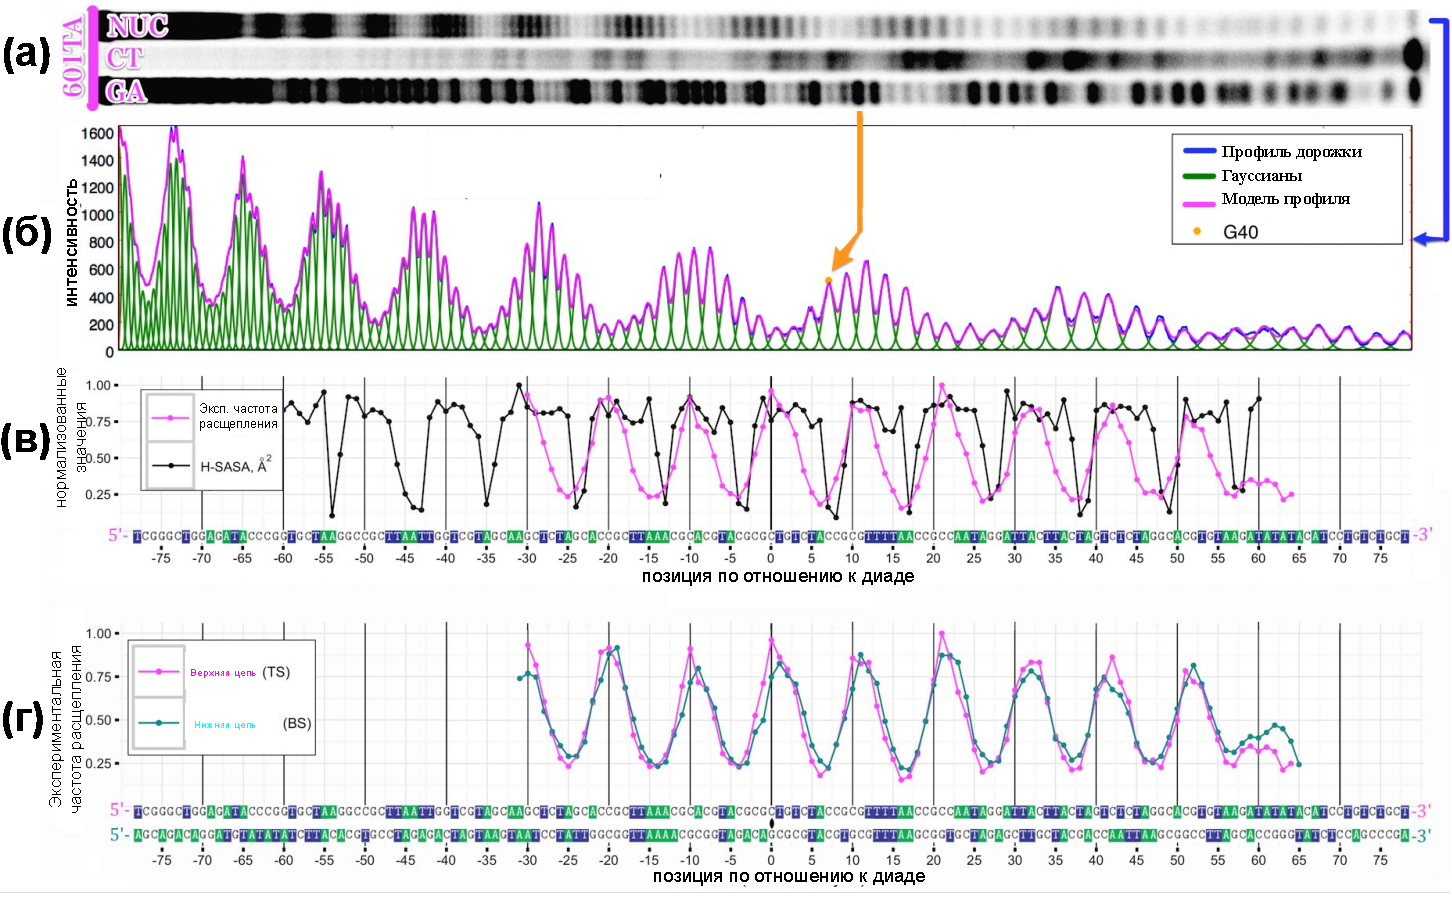
\includegraphics[width=\textwidth]{images/p5/part5_2_nar/p5_2_f5.pdf}
    \caption[Количественная оценка экспериментов по гидроксильному футпринтингу и сравнение с теоретическими профилями, полученными на основе атомной структуры (для нуклеосомы 601TA-NUC)]{Количественная оценка экспериментов по гидроксильному футпринтингу и сравнение с теоретическими профилями, полученными на основе атомной структуры (для нуклеосомы 601TA-NUC). (A) Исходное изображение геля ПААГЭ для сегментов ДНК, полученных с помощью гидроксильного футпринтинга нуклеосом, восстановленных на последовательности 601TA (NUC), и соответствующих продуктов реакции Максама-Гилберта (CT, GA). Данные показаны только для верхней цепи. (Б) соответствующий необработанный профиль интенсивности дорожек HRF, извлеченный из изображения геля, и его деконволюция в индивидуальные интенсивности полос путем подбора функций Гаусса; приводятся среднеквадратическое отклонение (RMSD) и относительное RMSD между исходным профилем и подобранной моделью; также указано RMSD для площади пика, площади пиков рассчитываются как площади под кривой между соседними минимумами. (В) суперпозиция количественных экспериментальных частот расщепления ДНК и профилей H-SASA, рассчитанных на основе атомистической структуры; оба профиля нормализованы до своих максимальных значений. (Г) Суперпозиция экспериментальных частот расщепления ДНК для верхней и нижней цепей ДНК в нуклеосоме 601TA-NUC}
    \label{fig:p5:p5_2_f5}
\end{figure}

\begin{figure}[H]
    \centering
    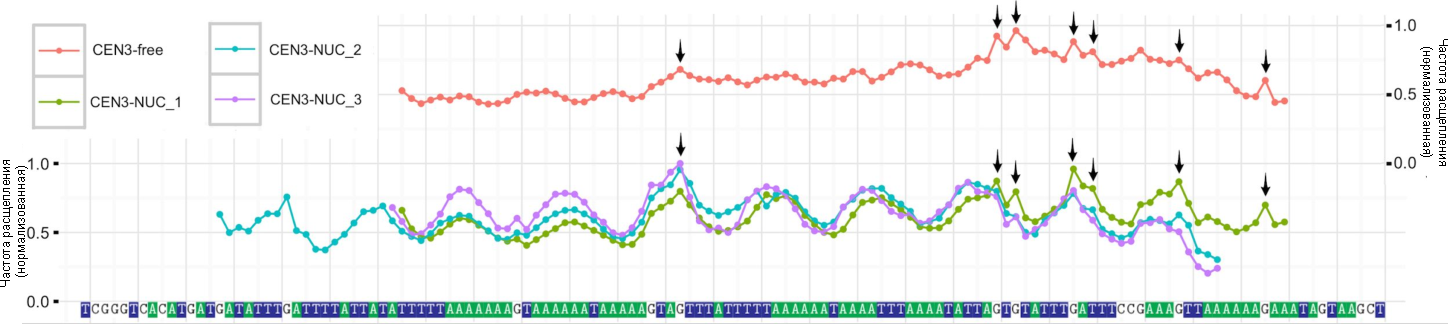
\includegraphics[width=\textwidth]{images/p5/part5_2_nar/p5_2_f6.pdf}
    \caption[Профили частоты расщепления ДНК для нуклеосом CEN3-NUC и ДНК свободной CEN3 ДНК]{Профили частоты расщепления ДНК для нуклеосом CEN3-NUC и ДНК свободной CEN3 ДНК. Данные нескольких экспериментов для верхней цепи объединены, стрелки указывают на незначительные всплески, видимые как на свободных, так и на нуклеосомных профилях ДНК, приписываемые зависимым от последовательности вкладам.}
    \label{fig:p5:p5_2_f6}
\end{figure}



\subsubsection{Моделирование нуклеосомы дрожжей CEN3 помощью интегративного подхода}
Мы использовали метод, описанный в предыдущем разделе, чтобы определить положение диады в восстановленной \textit{in vitro} центромерной нуклеосоме \textit{S. cerevisiae} из хромосомы III (CEN3-NUC) и построить ее структурную модель. С этой целью были проанализированы профили HRF для обеих нитей ДНК, полученные в результате трех независимых экспериментов (рисунок \ref{fig:p5:p5_2_f6}), в соответствии с предложенным нами методом. Мы проиллюстрируем применение нашего подхода к этому набору данных ниже. Были взяты образцы и протестированы различные предполагаемые положения диады нуклеосомы, как описано ранее. Специфическая интерес представляла область вблизи положения 64, которое, как предполагалось в более ранних экспериментах MNase-seq, была центром области устойчивости к расщеплению МНКазой \cite{cole_centromeric_2011}. Корреляционный анализ (рис. \ref{fig:p5:p5_2_f8}A и Б) выявил несколько возможных позиций диад с высокими уровнями корреляции между выровненными профилями (позиции 61,5, 67 и 72). Позиция 67 была отклонена как нарушающая соотношение ``правило 3:7'', что становится очевидным после просмотра выравнивания профилей HRF. Были еще две возможные позиции 61,5 и 72 с одинаковым соотношением коэффициента R = 0,78. Однако позиция 61,5 обеспечила лучшее соответствие между профилями верхней и нижней цепи ДНК в регионе вокруг диады (и, таким образом, ее можно считать лучшим кандидатом для расположения диады). Положение 61.5 расположено намного ближе к нашей исходной области интереса, основанной на оценке положения диады \textit{in vivo} (положение 64).
Все доступные рентгеновские структуры нуклеосом указывают на положение диады на конкретном нуклеотиде, а не между ними. В то же время, как обсуждалось ранее, среднее расположение диады в полуцелом положении возможно для ансамбля нуклеосом в растворе, особенно в случае палиндромных последовательностей. Анализ коэффициента корреляции указал на позицию 61 как более предпочтительную (рис. \ref{fig:p5:p5_2_f8}A), и ее в дальнейшем использовали для построения точной модели нуклеосомы CEN3-NUC (рис. \ref{fig:p5:p5_2_f8}В).
Знание точного местоположения диады позволяет впервые увидеть пространственные отношения между ключевыми элементами ДНК и белковыми элементами, которые определяют функцию центромерных нуклеосом у дрожжей. Как A-участки ДНК, так и ключевые остатки гистона Cse4p, как было показано ранее, являются критическими для функции центромеры у дрожжей, однако их коллективное взаимодействие остается не вполне понятным \cite{baker_genetic_2005,malik_major_2009}.

\begin{figure}[H]
    \centering
    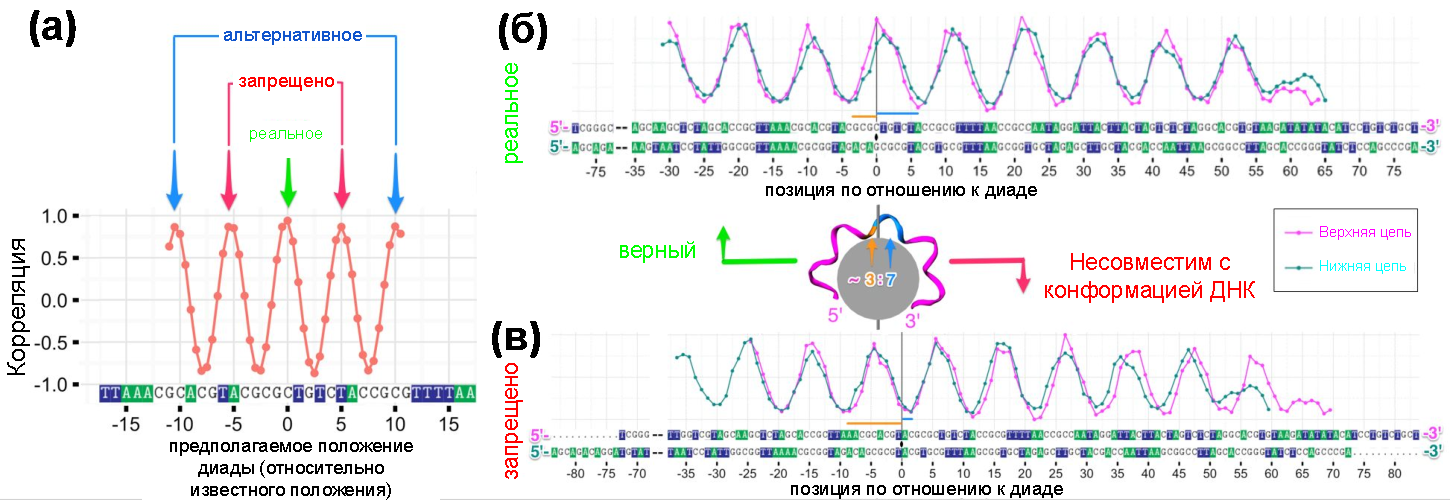
\includegraphics[width=\textwidth]{images/p5/part5_2_nar/p5_2_f7.pdf}
    \caption[Объяснение алгоритма идентификации диады применительно к нуклеосоме 601TA-NUC с известным положением диады]{Объяснение алгоритма идентификации диады применительно к нуклеосоме 601TA-NUC с известным положением диады. (A) Коэффициент корреляции Пирсона между экспериментальными профилями HRF верхней (TS) и нижней (BS) цепей ДНК как функция предполагаемого положения диады, используемого для выравнивания этих профилей. Реальное положение диады соответствует одному из локальных максимумов. Только половина локальных максимумов совместима со стереохимически допустимым решением (``правило 3: 7''). (Б) Наложение профилей TS и BS, выровненных с использованием реальной (известной) позиции диады. (В) Наложение профилей TS и BS, выровненных с использованием стереохимически запрещенного предполагаемого положения диады.}
    \label{fig:p5:p5_2_f7}
\end{figure}


\begin{figure}[H]
    \centering
    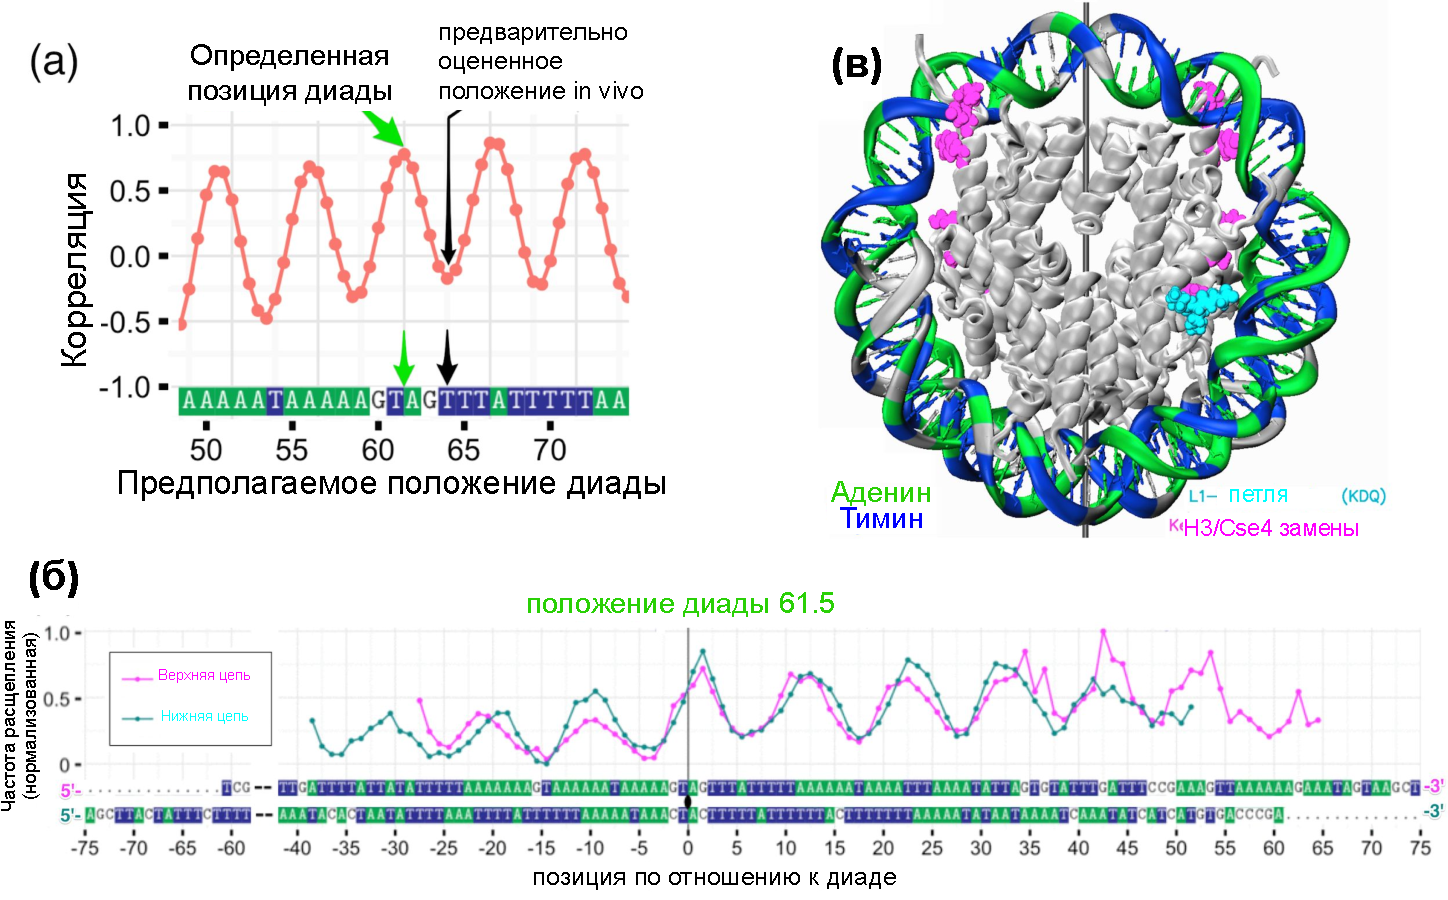
\includegraphics[width=\textwidth]{images/p5/part5_2_nar/p5_2_f8.pdf}
    \caption[Применение алгоритма идентификации диады  к нуклеосоме CEN3-NUC с неизвестным положением диады.]{Применение алгоритма идентификации диады  к нуклеосоме CEN3-NUC с неизвестным положением диады. (A) коэффициент корреляции Пирсона между экспериментальными профилями HRF верхней (TS) и нижней (BS) цепей ДНК как функция предполагаемого положения диады; показано положение диады, согласующееся с данными HRF (зеленая стрелка) и ранее оцененное \textit{in vivo} положение по устойчивости к расщеплению микрококовой нуклеазой (черная стрелка) \cite{cole_centromeric_2011}. (Б) Наложение профилей TS и BS, выровненных с использованием идентифицированной позиции диады. (В) Модель нуклеосомы CEN3-NUC, построенная с использованием положения ДНК, идентифицированного в экспериментах с HRF (диада установлена в положение 61). Нити ДНК окрашены в соответствии с их последовательностью, выделяя AT-участки: A –– зеленый, T –– синий, G или C –– серый.}
    \label{fig:p5:p5_2_f8}
\end{figure}



\subsection{Обсуждение}
В этой работе мы провели эксперименты по гидроксильному футпринтингу на двух нуклеосомных системах и разработали вычислительную основу для анализа данных HRF, полученных в результате экспериментов с нуклеосомами в растворе; интерпретации данных HRF путем сравнения с теоретическими профилями H-SASA; определения точного положение ДНК по данным HRF. Используя расширенный анализ структур нуклеосом, в сочетании с количественной оценкой экспериментальных данных HRF, мы смогли предложить интерпретацию экспериментов HRF на концептуально новом уровне. Это, в свою очередь, привело к развитию простого метода определения положения диады нуклеосом с разрешением в одну пару оснований. Мы использовали этот метод для определения положения диады в реконструированной \textit{in vitro} центромерной нуклеосоме \textit{S. cerevisiae} и для построения ее структурной модели. 
Алгоритм  идентификации диады, предложенный в этом исследовании, основан на соотношении симметрии между двумя цепями нуклеосомной ДНК. Мы показали, что это требование симметрии прямо выражается в сходстве профилей HRF верхней и нижней цепей ДНК. Использование этого критерия и экспериментальных данных для двух цепей ДНК повышает точность и надежность метода идентификации диады по сравнению с ситуацией, когда профиль HRF для каждой цепи анализируется отдельно. Последний подход до сих пор использовался в нескольких предыдущих исследованиях, которые в основном прибегали к сообщению приблизительного местоположения диады на ДНК \cite{hayes_structure_1990,widlund_nucleosome_1999,morozov_using_2009,ober_12-dgpg_2008,cannistraro_rapid_2015}. Идентификация положения диады с разрешением в одну пару оснований ранее достигалась сайт-направленным расщеплением гидроксильными радикалами или сайт-специфическим фотохимическим сшиванием \cite{flaus_mapping_1996,kassabov_high-resolution_2002}. Однако эти методы требуют химического включения определенных зондов в октамер гистонов в симметричных положениях, и диада затем определяется как средняя точка между реакционными сайтами. Метод, описанный в данной работе, обеспечивает разрешение в одну пару оснований с использованием обычных экспериментальных данных HRF без необходимости дорогостоящих модификаций гистонов. 
В качестве доказательства концепции мы оценили расположение ДНК в \textit{in vitro} нуклеосоме CEN3-NUC, которое оказалось на расстоянии ~ 3 п.н. от ранее оцененного положения \textit{in vivo} центра области, устойчивой к расщеплению микрококовой нуклеазе \cite{cole_centromeric_2011}. Точно определенное положение диады позволило нам построить модель этой нуклеосомы и выявить пространственную взаимосвязь между ориентацией последовательности ДНК и ключевыми белковыми мотивами белка Cse4p (Рисунок \ref{fig:p5:p5_2_f8}). Наша модель может служить основой для будущих исследований, направленных на понимание кооперативного взаимодействия и взаимодействия между белком Cse4p и A-траками последовательностей CEN центромер хромосом пекарских дрожжей.
В настоящее время известно, что последовательности CEN не консервативны между разными хромосомами у дрожжей, но наличие в их составе А-трактов имеет решающее значение для выживания \cite{baker_genetic_2005}. Однако молекулярный механизм(ы) вовлечения А-трактов в функцию центромеры дрожжей остается неясным. Одним из аспектов может быть особая геометрия ДНК, присущая А-трактам, которые известны своей конформационной жесткостью и узкими малыми бороздками как в свободной ДНК \cite{haran_unique_2009}, так и в нуклеосоме \cite{bao_nucleosome_2006}. В отличие от обычного гистона H3, вариант Cse4p не имеет остатка аргинина (замещенного серином R63S153), который в случае H3 вставлен в малую бороздку ДНК около положения $\pm$ 15. Известно, что это положение примыкает к уникальному гистоновому мотиву, который формирует чрезвычайно узкую малую бороздку через гидрофобный ``сахарный зажим'' \cite{wu_structural_2010}. С другой стороны, известно, что мотивы TnAn (в отличие от AnTn и в отличие от A-трактов) обнаруживают расширенные малые бороздки на динуклеотидах TpA \cite{stefl_dna_2004}. Последовательности CEN с высоким содержанием AT обычно имеют несколько A-трактов, которые разделены динуклеотидами TpA, и, таким образом, последовательности CEN также содержат несколько TnAn-подобных мотивов. Эти мотивы могут способствовать функционально важному расширению малой бороздки на соответствующих участках.
Интересно, что согласно нашей структурной модели центромерной нуклеосомы, последовательность CEN3 является квазипалиндромной рядом с определенным положением диады 61,5. Последовательность AAAGTAGTTT, обнаруженная на диаде, может быть преобразована в идеальный палиндром с заменой только 1 нуклеотида. Кроме того, 4 нуклеотида в диаде (GTAG) фланкированы сегментами ДНК, состоящими исключительно из A или T, богатых A-участками. Эти структурные данные могут дополнительно обеспечить понимание структуры центромерных нуклеосом и функционального связывания с ключевыми кинетохорными белками, такими как дрожжевой Mif2 (человеческий CENP-C), который предпочтительно связывается с AT-богатыми ДНК центромерных нуклеосом дрожжей (Xiao et al., Неопубликованные данные).

Помимо определения положения диады, эксперименты HRF могут быть использованы для дальнейшего углубления нашего понимания конформации ДНК в нуклеосомах. Возможность сделать это, однако, зависит от нашей способности сопоставить форму профилей HRF со структурными деталями нуклеосомы. Понимание расхождений между теоретически полученными профилями H-SASA и экспериментальными профилями HRF для известных структур является важным шагом в этом направлении. Наш сравнительный анализ профилей H-SASA и экспериментальных профилей показал, что, хотя их общая периодичность схожа, экспериментальные профили намного более гладкие и могут иметь разную величину и / или точное расположение максимумов и минимумов. Разница между теоретическими и экспериментальными профилями также была замечена в предыдущем исследовании комплекса ДНК-ТВР: значения H-SASA для некоторых нуклеотидов были близки к нулю, в то время как определенное количество расщеплений все же было обнаружено экспериментально \cite{pastor_detailed_2000}. Значительная вероятность расщепления ДНК на сайтах связывания ДНК может быть результатом нелинейной зависимости частоты расщепления от доступности растворителю. Фактически, предыдущие исследования показали обнаруживаемые вероятности расщепления за счет отрыва атомов водорода с исчезающе малой SASA \cite{balasubramanian_dna_1998}. Тем не менее, существенный вклад, вероятно, исходит от нуклеосомной динамики и конформационной неоднородности \cite{rychkov_partially_2017,winogradoff_shearing_2015}. Нуклеосомная ДНК в растворе принимает ряд состояний с твист-дефектом ДНК \cite{edayathumangalam_nucleosomes_2005}. В течение HRF экспериментов ансамбль нуклеосом в растворе с различными конформациями будет доступен для гидроксилрадикальной атаки. Дополнительные конформационные вариации также могут быть результатом различий в позиционировании ДНК \cite{widom_role_2001}.

Одним из важных аспектов является появление идентифицируемых локальных максимумов на экспериментальном профиле на расстоянии 10–11 п.н. - по одному на виток нуклеосомной ДНК, тогда как в профилях H-SASA 7–8 нуклеотидов ДНК витка почти одинаково доступны. Возможное объяснение может исходить из несовершенства модели H-SASA, служащей приближением сложной физики и химии разрыва ДНК. В частности, как подчеркивают Бегусова и др. контролируемая диффузией природа реакции атаки гидроксильных радикалов и быстрый распад радикалов из-за взаимодействия с другими атомами должны сделать вероятность разрыва зависимой не только от локальной доступности атомов водорода, но и от общей формы молекулы, которая будет управляют потоком радикалов, которые могут достичь заданного участка ДНК из раствора \cite{begusova_radack_2001,begusova_radiolysis_2000}. Более того, необходимо учитывать распределение электронной плотности целевой молекулы, чтобы правильно описать реакцию атаки гидроксильных радикалов. Различные многоступенчатые реакционные пути могут также вносить вклад в химическую сложность, например, сообщалось о механизмах расщепления ДНК посредством вторичных гистоновых радикалов \cite{zhou_dna_2014}.

С момента пионерских исследований лабораторий Вольфа и Туллиуса в начале 1990-х годов по периодичности нуклеосомной ДНК в растворе на основе экспериментов HRF \cite{hayes_structure_1990,hayes_histone_1991,hayes_histone_1991-1,bashkin_structure_1993} стали доступны рентгеновские структуры нуклеосом с высоким разрешением \cite{luger_crystal_1997}. Периодичность ДНК в нуклеосомах является важным параметром из-за ее влияния на сверхспирализацию ДНК \cite{klug_helical_1981}. Наше исследование, путем одновременного анализа профилей rTw, H-SASA и экспериментальных профилей HRF, позволяет изучить теоретические основы использования экспериментов HRF для определения периодичности ДНК. Результаты нашего анализа в настоящее время требуют осторожности при использовании положений максимумов или минимумов на экспериментальных профилях частоты расщепления ДНК для измерения периодичности нуклеосомной ДНК с высокой точностью (лучше, чем 1 п.н. / оборот). Как мы показали, минимумы профилей на профилях rTw и H-SASA не всегда совпадают, а положения минимумов могут отличаться на 1-2 п.н. из-за вариаций в локальных взаимодействиях гистон-ДНК. С другой стороны, максимумы на экспериментальных профилях частоты расщепления ДНК могут зависеть от локальной динамики ДНК, природы допустимых дефектов кручения, других динамических эффектов, а также некоторых нерегулярностей расщепления, специфичных для последовательности (локальные пики, как показано на рисунке \ref{fig:p5:p5_2_f8}). Кроме того, второстепенные, медленно мигрирующие продукты расщепления ДНК могут исказить форму профилей. Дальнейшие исследования могут выявить вклад этих эффектов в мельчайшие детали формы профилей HRF.

В совокупности наше исследование обеспечивает новый надежный подход к анализу и интерпретации данных экспериментов по расщеплению ДНК нуклеосом гидроксильными радикалами, определению положения ДНК с точностью до одной пары оснований и построению высокоточных молекулярных моделей неизвестных нуклеосом. Такие модели позволяют обнаружить уникальное пространственное расположение между гистонами и особенностями последовательностей ДНК и могут формировать рациональную основу для структурного понимания взаимодействий между нуклеосомами и другими белками хроматина. Учитывая аналогию между HRF и окислительным повреждением ДНК в клетках, результаты этого исследования могут быть в дальнейшем использованы для обоснования влияния нуклеосом на повреждение ДНК с высоким разрешением.



\subsection{Благодарности}
Мы благодарим Т. Туллиуса за ценные предложения, которые помогли сформулировать идею этого исследования, и Л. Заславского за обсуждения оптимальных алгоритмов подбора данных.
Исследования были поддержаны программой очных исследований Национальной медицинской библиотеки и Национального института рака, Национальных институтов здоровья, США; Российским научным фондом [14–24-00031] (договор № 14-24-00031-р, разработка алгоритмов визуализации нуклеосом); Исследовательским кампусом Джанелия Медицинского института Говарда Хьюза;  Университетом Джона Хопкинса; программой сотрудничества США-России в области биомедицинских наук.





\section{Выводы главы \ref{part5_hrf}}
Создано программное обеспечение для оцифровки результатов гель-электрофореза продуктов расщепления ДНК с помощью гидроксильных радикалов. Данный подход позволяет количественно описывать интенсивность расщепления ДНК по каждому конкретному нуклеотиду. Разработаны подходы для оценки вероятности расщепления ДНК в заданных позициях на основе анализа доступности атомов водорода дезоксирибозы в молекулярных моделях, что позволяет использовать данные футпринтинга для задач интегративного моделирования. На основе данных подходов создан метод, позволяющий по данным футпринтинга ДНК определять с точностью до одного нуклеотида положение последовательности ДНК на нуклеосоме. Метод использован при создании модели центромерной нуклеосомы \textit{S. cerevisiae}.

Данные гидроксильного футпринтинга ДНК могут быть эффективно использованы для построения структурных моделей ДНК-белковых комплексов. Для ДНК-белковых комплексов, обладающих осью симметрии второго порядка, сравнение профилей расщепления ДНК для двух цепей позволяет дополнительно повысить точность определения положения ДНК относительно белка. 

% \subsection{Положения выносимые на защиту}
% %положения выносимые на защиту
% \begin{enumerate}
%   \item Разработан комплексный подход и программное обеспечение, позволяющие использовать экспериментальные данные по расщеплению ДНК гидроксил радикалами для построения атомистических моделей ДНК-белковых комплексов.
%   \item Разработан метод создания атомистических моделей нуклеосом, в которых позиционирование ДНК определяется на основе данных по расщеплению ДНК гидроксил радикалами.
% \end{enumerate}